\chapter{From Theory to Practice: Technical Design and Pilot Implementation}
\label{cha:chapter_5}

Having established a comprehensive theoretical and methodological foundation in the preceding chapters, this chapter transitions from conceptual frameworks into concrete system implementation. Specifically, it demonstrates the practical viability and flexibility of the developed generic \ac{dpp} system design model through a proof-of-concept pilot project. The implemented pilot architecture operationalizes an \acrlong{aas} (\acrshort{aas})-based digital twin to dynamically and automatically derive structured \ac{dpp}s, focusing on satisfying the main requirements identified in this research. \Cref{sec:pilot_architecture} of the chapter explains the precise derivation of the selected architectural configuration from the morphological analysis and decision logic model defined earlier. The subsequent \Cref{sec:pilot_implementation} then thoroughly examines and showcases the technical realization of the pilot, covering backend and frontend infrastructure, core modular components, and user interfaces.

\section{Pilot Architecture}
\label{sec:pilot_architecture}
The pilot implementation presented in this chapter is based directly upon the generic \ac{dpp} architecture model developed through morphological analysis conducted in \Cref{sec:generic_system_design_model}. Here, the rationale behind each selected architectural dimension and option will be briefly revisited and justified, highlighting explicit connections with empirical insights from the industry analysis (\Cref{sec:data_analysis}), expert interviews (\Cref{sec:expert_insights_evaluation}), and identified system requirements (\Cref{sec:regulatory_landscape}).

\Cref{tab:morphological_box_pilot} illustrates the morphological box presented previously (see \Cref{tab:morphological_box_dpp}), explicitly highlighting the architectural configuration selected for this proof-of-concept implementation.

\begin{table}[!t]
    \centering
    \caption{Selected Architecture Configuration for Pilot \ac{dpp} System}
    \renewcommand{\arraystretch}{1.2}
    \small
    \setlength{\emergencystretch}{3em}
    \begin{tabularx}{\linewidth}{|>{\centering\arraybackslash}m{3.5cm}|*{4}{>{\centering\arraybackslash}X|}}
        \hline
        \cellcolor{myDarkBlue}\textcolor{white}{\textbf{Dimension}} &
        \multicolumn{4}{c|}{\cellcolor{myDarkBlue}\textcolor{white}{\textbf{Options}}} \\
        \hline

        \cellcolor{myGrey}\textbf{Data Storage Model} & \cellcolor{myLightBlue}\textcolor{white}{Centralized} &
        Federated & Decentralized &
        -- \\ \hline

        \cellcolor{myGrey}\textbf{Storage Solution} &
        \cellcolor{myLightBlue}\textcolor{white}{Relational DB} &
        Document DB &
        Graph DB &
        Distributed Ledger \\ \hline

        \cellcolor{myGrey}\textbf{Ledger Technology} &
        \cellcolor{myLightBlue}\textcolor{white}{None} &
        Permissioned Blockchain &
        Permissionless Blockchain &
        DAG based \ac{dlt} \\ \hline

        \cellcolor{myGrey}\textbf{Data Model} &
        \cellcolor{myLightBlue}\textcolor{white}{Relational Schema} &
        \cellcolor{myLightBlue}\textcolor{white}{JSON Document} &
        Knowledge Graph &
        -- \\ \hline

        \cellcolor{myGrey}\textbf{Governance Structure} &
        \cellcolor{myLightBlue}\textcolor{white}{Central Authority} &
        Service Providers &
        Self Sovereign &
        -- \\ \hline
        
        \cellcolor{myGrey}\textbf{Digital Twin} &
        \cellcolor{myLightBlue}\textcolor{white}{Yes} &
        No &
        -- &
        -- \\ \hline

        \cellcolor{myGrey}\textbf{Semantic Model} &
        \cellcolor{myLightBlue}\textcolor{white}{\ac{aas} Schema} &
        UNTP Schema &
        Proprietary Schema &
        -- \\ \hline

        \cellcolor{myGrey}\textbf{Resolver Architecture} &
        \cellcolor{myLightBlue}\textcolor{white}{None} &
        Single Resolver &
        Tiered Resolver &
        Distributed Resolver \\ \hline

        \cellcolor{myGrey}\textbf{Regulatory Scope} &
        \cellcolor{myLightBlue}\textcolor{white}{\ac{espr}} &
        Sector-specific &
        Global  &
        -- \\ \hline

        \cellcolor{myGrey}\textbf{Authentication} &
        \cellcolor{myLightBlue}\textcolor{white}{Centralized IAM} &
        Decentralized \ac{did} &
        -- &
        -- \\ \hline

        \cellcolor{myGrey}\textbf{Access Control} &
        \cellcolor{myLightBlue}\textcolor{white}{\ac{rbac}} &
        ABAC &
        Smart Contracts &
        -- \\ \hline

        \cellcolor{myGrey}\textbf{Data Exchange Protocol} &
        \cellcolor{myLightBlue}\textcolor{white}{REST \ac{api}} &
        GraphQL &
        Event driven &
        Proprietary \\ \hline

        \cellcolor{myGrey}\textbf{Data Query Protocol} &
        \cellcolor{myLightBlue}\textcolor{white}{None} &
        GraphQL &
        SPARQL &
        -- \\ \hline

        \cellcolor{myGrey}\textbf{Data Update Pattern} &
        Batch &
        \cellcolor{myLightBlue}\textcolor{white}{Event-driven} &
        Real-time &
        -- \\ \hline

        \cellcolor{myGrey}\textbf{Lifecycle Coverage} &
        Cradle-to-Gate &
        \cellcolor{myLightBlue}\textcolor{white}{Full Lifecycle} &
        End-of-Life Only &
        -- \\ \hline

        \cellcolor{myGrey}\textbf{Security \& Trust} &
        \cellcolor{myLightBlue}\textcolor{white}{Standard Cryptography} &
        Verifiable Credentials &
        PETs &
        -- \\ \hline

        \cellcolor{myGrey}\textbf{Scalability Infrastructure} &
        \cellcolor{myLightBlue}\textcolor{white}{Cloud-native} &
        Edge Computing &
        Blockchain Scalability &
        -- \\ \hline

        \cellcolor{myGrey}\textbf{AI Integration} &
        AI Components Integrated &
        \cellcolor{myLightBlue}\textcolor{white}{No AI Integration}
        & --
        & --
        \\ \hline

        \cellcolor{myGrey}\textbf{Data Carrier Technology} &
        \cellcolor{myLightBlue}\textcolor{white}{\ac{qr} Code} &
        \ac{rfid} &
        \ac{nfc} &
        Other \\ \hline

        \cellcolor{myGrey}\textbf{User Interaction Layer} &
        Mobile Application &
        \cellcolor{myLightBlue}\textcolor{white}{Web Application} &
        \ac{api} only &
        -- \\ \hline
    \end{tabularx}
    \label{tab:morphological_box_pilot}
\end{table}

This specific configuration was selected by following the decision pathway (see \Cref{fig:dpp_generic_model}) through the dimensions of the morphological box and decision logic graph.

\textbf{Data Storage Model and Governance Structure:}
For the pilot, a centralized storage model was selected. This decision is justified by the objective of achieving simplicity, easier data management, and a controlled proof-of-concept environment. Correspondingly, a central authority governance structure was chosen to reflect a realistic yet manageable administrative scenario, aligning closely with insights from expert interviews suggesting centralized governance models as initial implementation patterns before scaling into federated or decentralized architectures. Notably, despite the centralized model used in the pilot, the system's inherent modularity, flexibility, and interoperability ensure that alternative storage and governance structures can be easily integrated. This design choice enables the system to be efficiently adapted or expanded to support federated, decentralized, or hybrid architectures in future iterations.

\textbf{Ledger Technology, Authentication, and Access Control:}
Given the selected centralized governance, the implementation excluded distributed ledger technologies to avoid unnecessary complexity, following compatibility constraints identified in \Cref{sec:generic_system_design_model}. Consequently, the system employs a centralized Identity and Access Management (IAM) system, utilizing JSON Web Token (JWT) authentication combined with \acrlong{rbac}. This configuration directly aligns with industry practices identified in expert interviews, favoring simplicity and operational clarity.

\textbf{Storage Solution and Data Model:}
A relational database was selected as the foundational storage technology, utilizing a hybrid data model that integrates structured relational schemas with JSON document columns. This approach leverages the strengths of both worlds—combining the relational model's robust ability to define clear, consistent, and reliable relationships between entities with JSON's flexibility and semantic expressiveness. By embedding JSON columns within a relational schema, the system efficiently stores precise semantic representations while maintaining strong relational integrity. This hybrid model provides essential portability and adaptability, aligning with the requirements identified by \textcite{Jansen.2023} (see \Cref{tab:dpp_requirements}) and confirmed through the expert interviews.

\textbf{Digital Twin and Semantic Model:}
The pilot adopts an \ac{aas}-based digital twin model based on the extensive literature review, specifically the research into \ac{aas}‐based \ac{dpp} solutions by \textcite{Kuhn.2025, Pourjafarian.2023} (see \Cref{sec:technology_review}), as well as insights from Experts 3 and 5 (see \Cref{sec:expert_insights_evaluation}) emphasizing the digital twin as a foundational enabler for frictionless \ac{dpp} generation. Moreover, endorsed by standardization bodies such as the \ac{idta}, the \ac{aas} has emerged as a leading digital twin approach due to its structured, modular, and extensible schema. By leveraging the \ac{aas} as a semantic model, the pilot ensures high interoperability among diverse stakeholders and systems, facilitating both real-time data exchange and comprehensive product lifecycle management. This alignment between the \ac{aas}’s technological strengths and core \ac{dpp} requirements, reinforced by academic research and industry testimony, makes it the ideal centerpiece of the pilot architecture. Once a comprehensive digital twin is established, generating machine‐readable \ac{dpp}s becomes a streamlined extension of the same ecosystem, further highlighting how the \ac{aas} can serve as the backbone of robust \ac{dpp} solutions.

\textbf{Regulatory Scope and Lifecycle Coverage:}
This thesis follows the \acrlong{eu}’s leading regulatory framework for \ac{dpp}s, the \ac{espr}, which currently offers the most comprehensive standards for \ac{dpp} adoption. By mandating full lifecycle visibility, the \ac{espr} establishes a rigorous scope aligned with \acrlong{ce} goals. Addressing these requirements, the \ac{aas} serves as a robust digital twin technology capable of tracking product data from cradle to end of life. Consequently, following the \ac{espr}’s far-reaching directives with the \ac{aas}’s holistic lifecycle coverage results in a comprehensive, compliant and forward-looking \ac{dpp} implementation.

\textbf{Data Update Pattern, Data Exchange, and Query Protocols:}
An event-driven data update pattern was chosen to dynamically and responsively manage data changes within the centralized architecture without excessive complexity. For data exchange, REST \ac{api}s were selected due to their simplicity, industry-wide acceptance, and inherent compatibility with JSON-based data interactions. Given the direct REST-based data retrieval and a relational JSON-hybrid data model, a dedicated data query protocol was deemed unnecessary.

\textbf{Resolver Architecture and Scalability Infrastructure:}
Considering the pilot's limited scope and centralized data management strategy, no explicit resolver architecture was implemented. However, ensuring scalability remained paramount, leading to the use of cloud-native technologies, containerized deployment, and a flexible proxy layer for dynamic routing and load balancing. Such a configuration is capable of easily scaling into a bigger federated system.

\textbf{User Interaction Layer, Data Carrier Technology, and AI Integration:}
To maintain clear modularity, these components were designed to operate independently from core system logic. A web-based user interface ensures intuitive interaction, while QR code technology was chosen as the data carrier method, reflecting the ubiquitous adoption observed in industry practice (see \cref{fig:initiatives_data_carrier}). AI integration was excluded at this stage to maintain a clear focus on core architectural validation.

The configuration described above, justified through systematic alignment with empirical insights and compatibility constraints, ultimately resulted in an internally consistent, flexible, and practically viable proof-of-concept \ac{dpp} architecture that effectively demonstrates the principles of interoperability, modularity, and adaptability.

\begin{figure}[htbp]
  \centering
  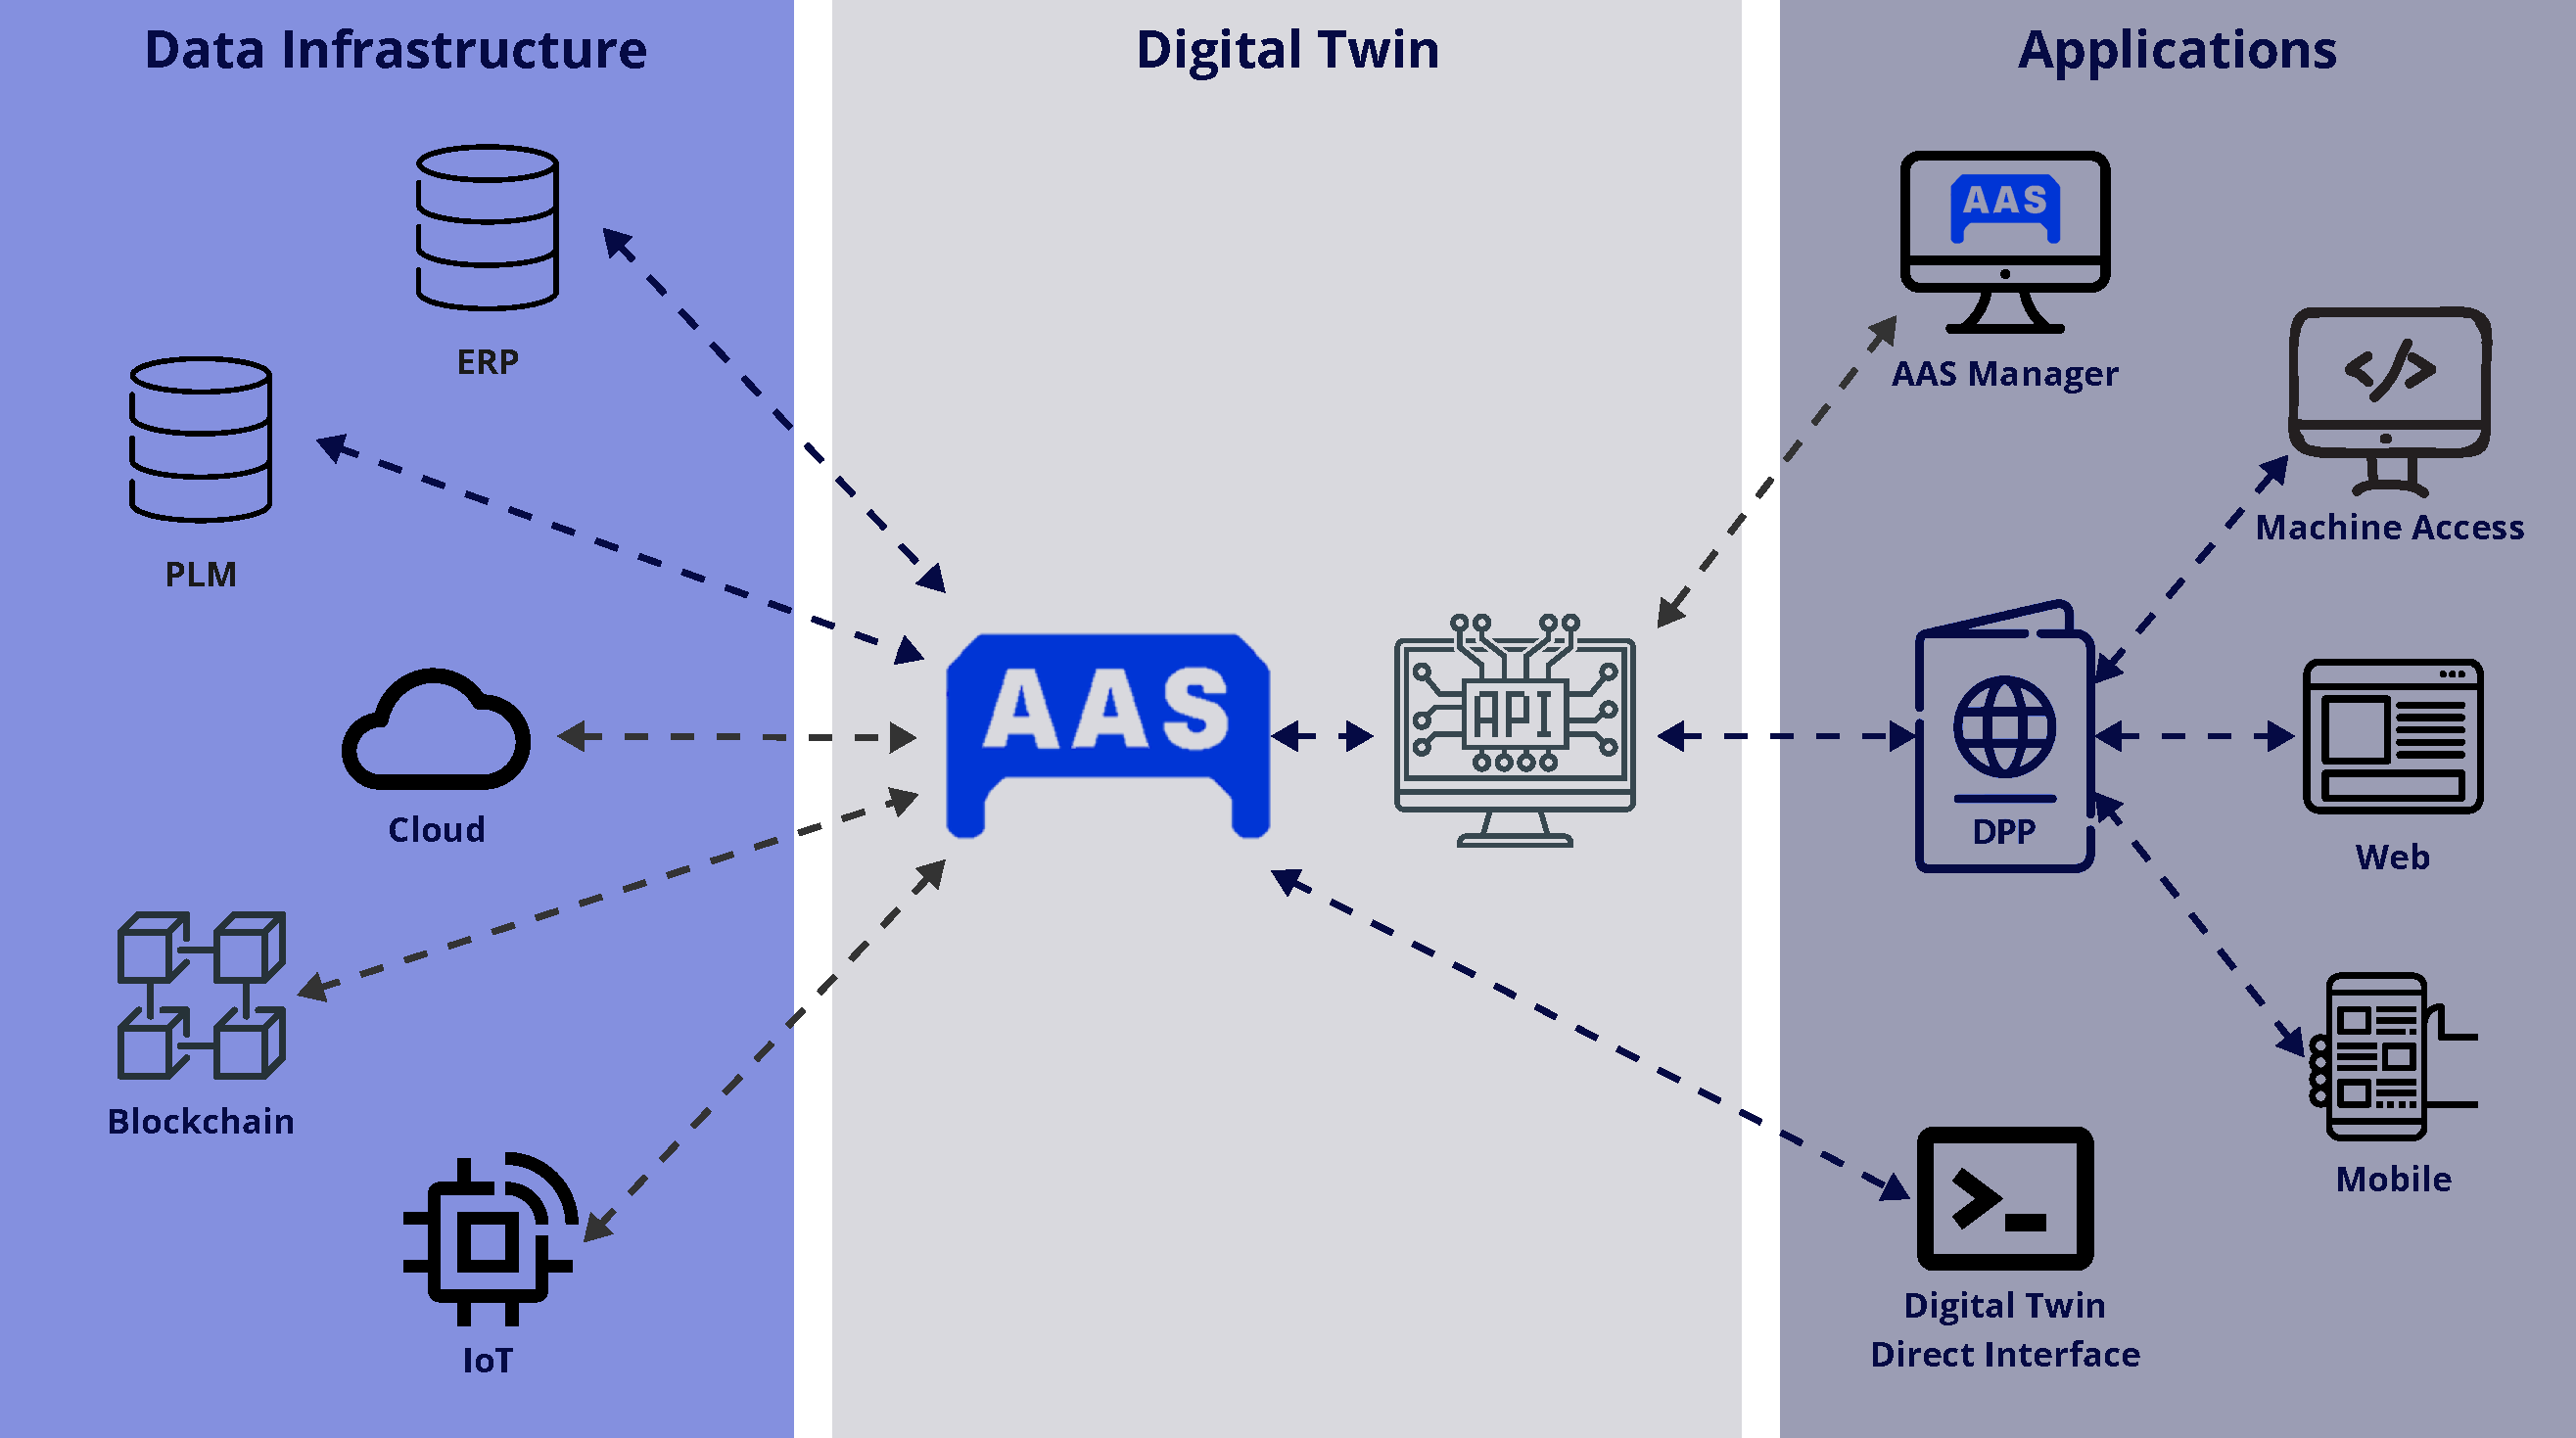
\includegraphics[width=\textwidth]{figures/pilot_architecture_global.pdf}
  \caption{%
    \textit{Pilot Architecture Overview} 
  }
  \label{fig:pilot_architecture_global}
\end{figure}

\Cref{fig:pilot_architecture_global} depicts the pilot system’s conceptual architecture in direct alignment with the three‐layer \ac{dpp} framework outlined in \Cref{sec:dpp_concept_architecture}. At the core, the Digital Twin (embodied by the \ac{aas}) functions as the “glue” that unifies heterogeneous product data sources in the Data Layer. In the proposed architecture, the Digital Twin encapsulates the \ac{aas} within a dedicated backend infrastructure, thereby forming the Processing \& Governance Layer and enforcing standardized governance and interoperability. Through this central integration, the structured product data passes through a dedicated \ac{dpp} mapping mechanism to efficiently package information into standardized, machine‐readable passport representation. This low‐friction \ac{dpp} representation can then be seamlessly consumed and presented by various consumer‐facing applications in the User \& Application Layer. In this manner, the pilot architecture demonstrates how a robust digital twin not only streamlines data consolidation and regulatory compliance but also accelerates \ac{dpp} generation for widespread, interoperable industry use.

\section{Pilot Implementation}
\label{sec:pilot_implementation}

Having presented a high-level conceptual architecture in the previous section, this section thoroughly describes the detailed technical implementation of the \ac{dpp} pilot system. \Cref{fig:pilot_architecture_technical} provides a detailed technical diagram of the implemented pilot system, explicitly identifying concrete technologies, components, and interactions among them.

\begin{figure}[htbp]
  \centering
  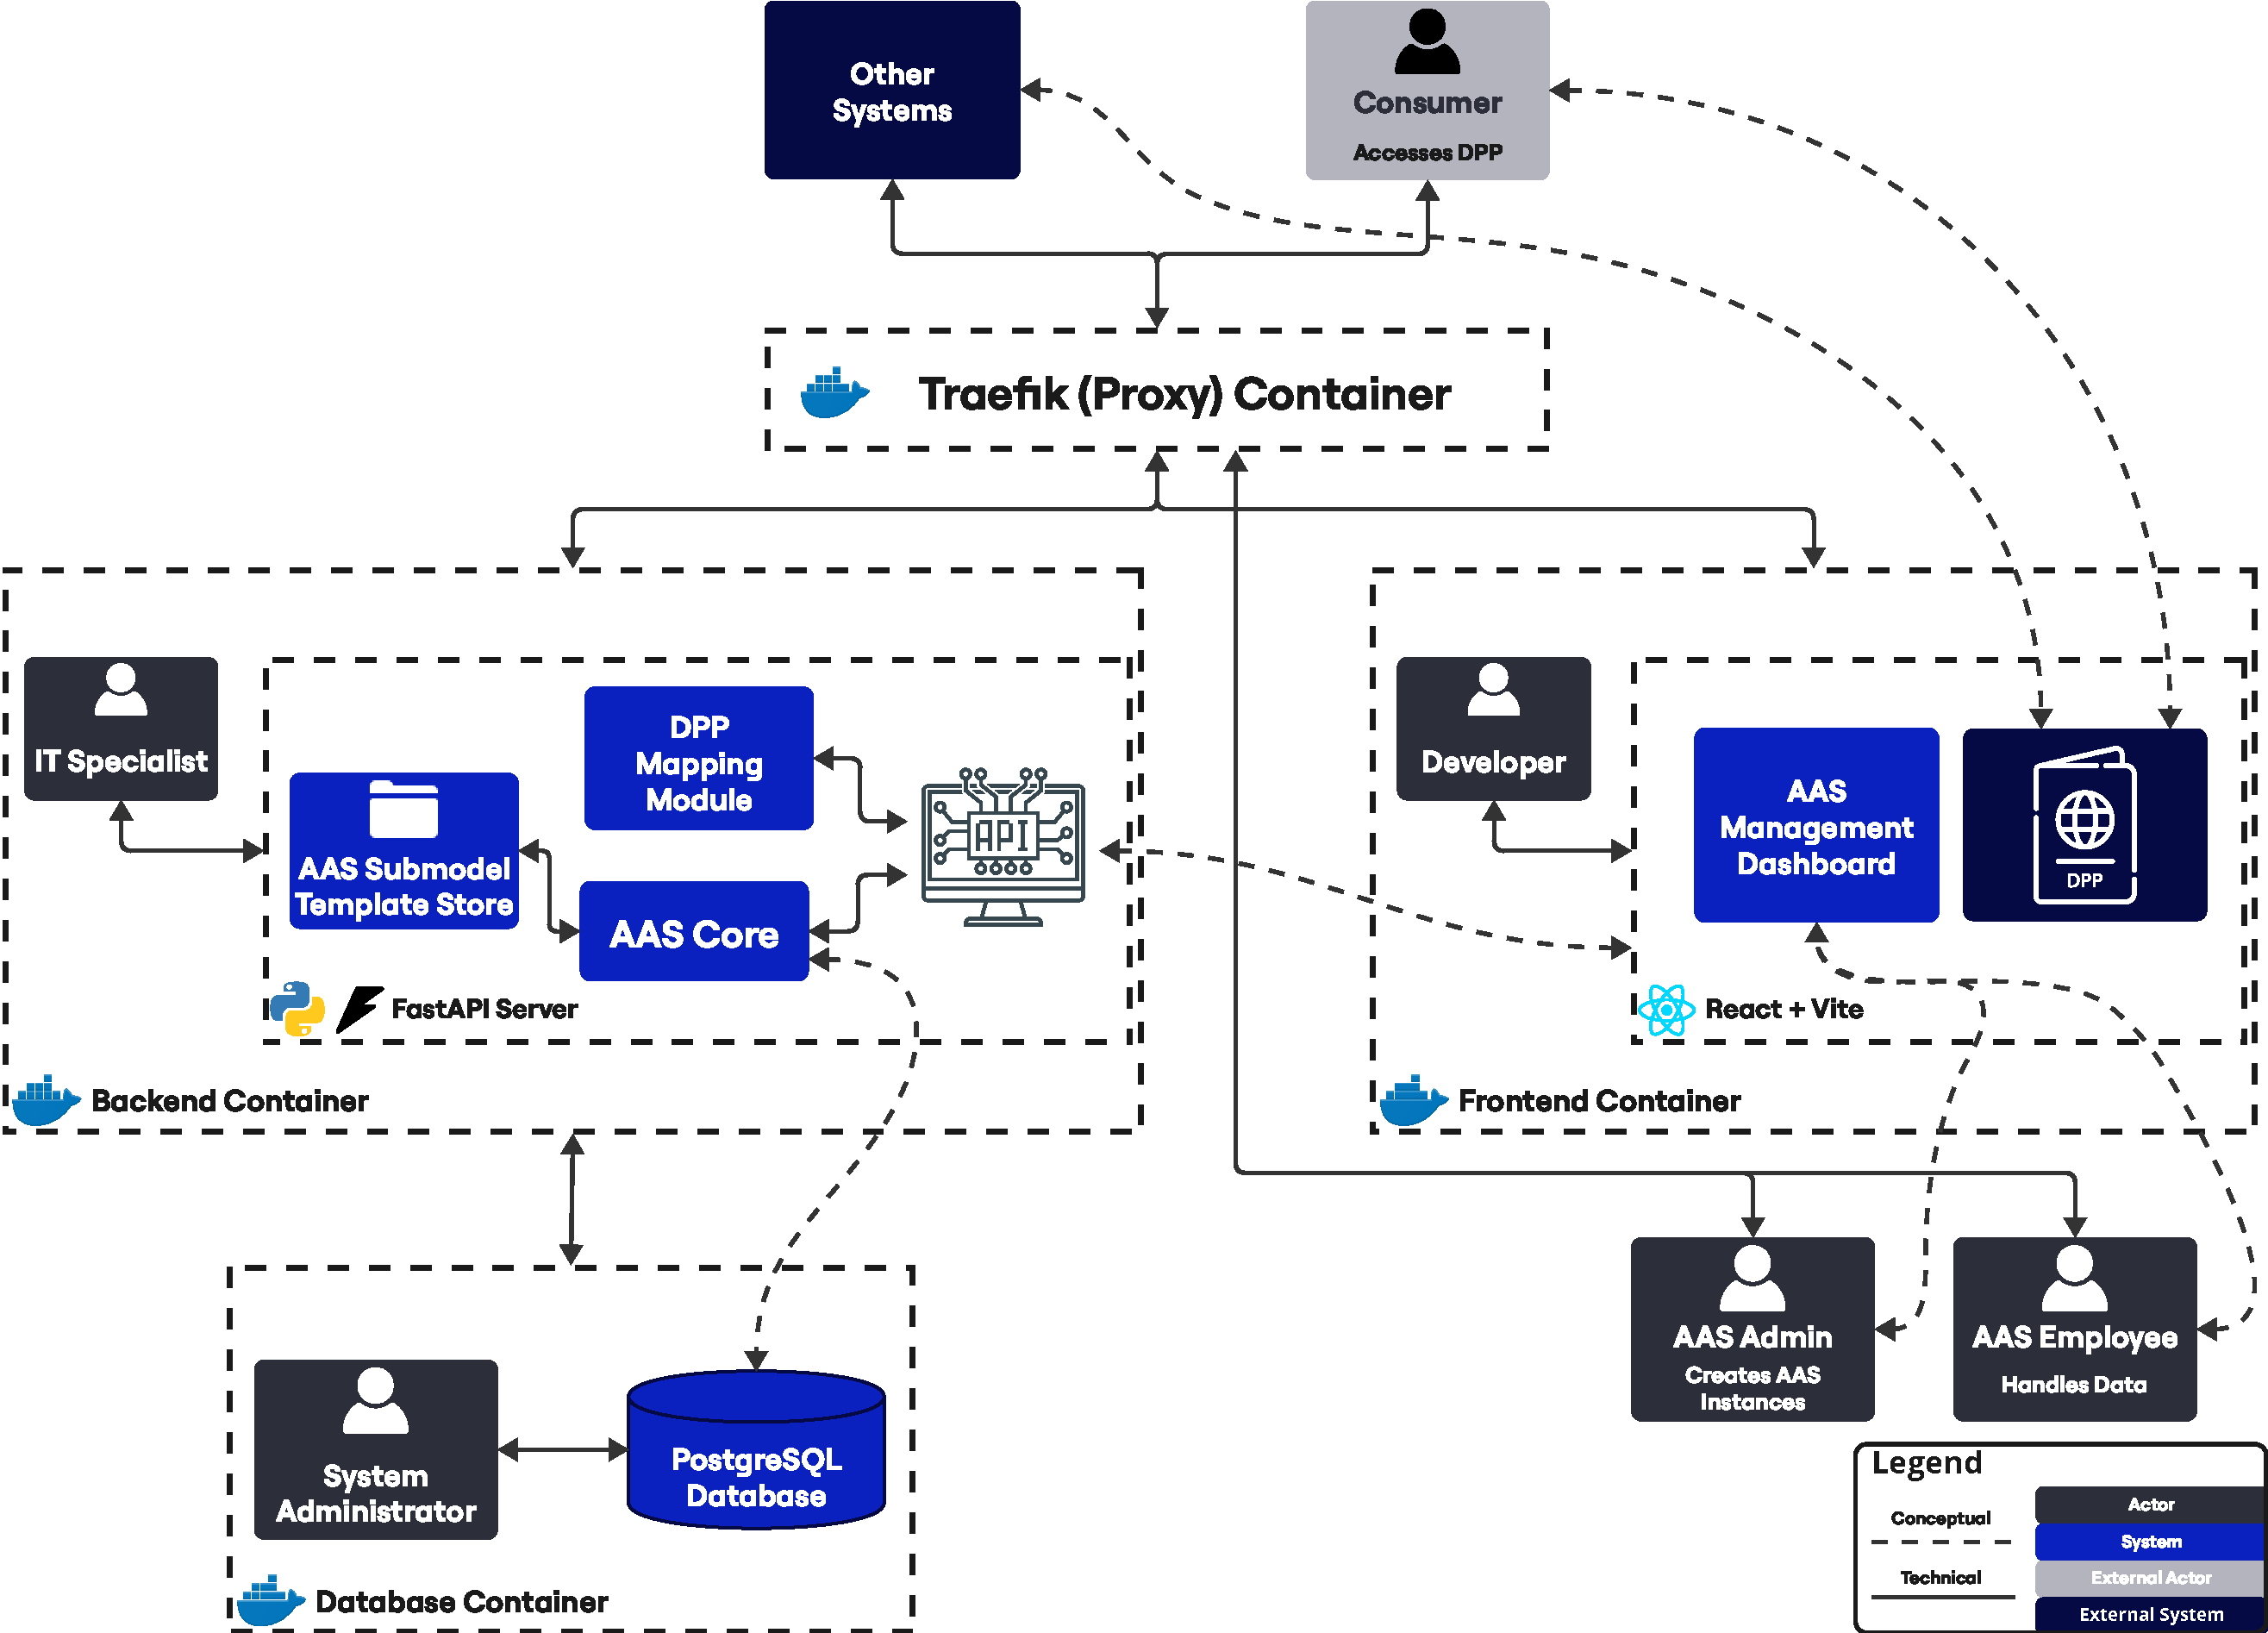
\includegraphics[width=\textwidth]{figures/pilot_architecture_technical.pdf}
  \caption{%
    \textit{\ac{dpp} Pilot: Detailed Technical Diagram} 
  }
  \label{fig:pilot_architecture_technical}
\end{figure}

At the system’s core, the architecture is designed for modularity, scalability, and ease of maintenance, facilitated by the strategic adoption of containerization technologies and modern web development frameworks. The following section comprehensively elaborates on each major component, clarifying its functional role and technological context within the overall architecture.

\subsection{Technology Stack}

\textbf{Containerized Deployment with Docker and Docker Compose:}
The entire architecture is built upon containerization technology using Docker, an open-source platform for packaging, distributing, and running applications consistently across diverse computing environments \autocite{DockerInc..n.d.}. Docker Compose extends this capability by defining multi-container applications, orchestrating backend, frontend, database, and proxy services for both development and production deployments \autocite{DockerInc..n.d.b}.

\textbf{Reverse Proxy and Load Balancer (Traefik):}
All incoming requests are first managed by the Traefik reverse proxy, a dynamic, container-native load balancer and reverse proxy solution. Traefik enables automatic service discovery, dynamic configuration, and seamless SSL certificate management, ensuring secure and scalable HTTPS communication across the frontend, backend, and external-facing \ac{api}s. \autocite{TraefikLabs.n.d.}

\textbf{Backend Infrastructure (FastAPI, PostgreSQL, JWT, and RBAC):}
The backend application is developed using Python, a widely-adopted, versatile programming language known for its stability, readability, ease of use, and strong community support \autocite{PythonSoftwareFoundation.n.d.}. The backend \ac{api} leverages FastAPI, a modern, high-performance web framework specifically designed for building scalable \ac{api}s with Python. FastAPI provides automatic interactive \ac{api} documentation, validation, and serialization via Pydantic models, as well as support for asynchronous programming paradigms \autocite{Ramirez.n.d.}. Data persistence and structured storage are managed by PostgreSQL, a powerful, open-source relational database system that provides reliability, robustness, and support for both traditional relational data and modern JSON document storage capabilities, facilitating the combined relational and JSON-based data modeling utilized in this pilot \autocite{ThePostgreSQLGlobalDevelopmentGroup.n.d.}.

Authentication and user authorization are secured using JSON Web Tokens (JWT), an open industry standard for securely transmitting claims between parties \autocite{Jones.2015}. The implementation ensures secure, stateless, and scalable session management. Access control is enforced through a structured \acrlong{rbac} (\acrshort{rbac}) system, where permissions are clearly defined per role, allowing precise data and interface restrictions based on user roles \autocite{Ferraiolo.1992}.

\textbf{\ac{aas} Core via Eclipse BaSyx:}
Central to the \ac{dpp} pilot system's architecture is the implementation of the \acrlong{aas}, an integral concept of Industry 4.0 and digital twin frameworks as elaborated in \Cref{sec:technology_review}. To realize this core component, the architecture leverages Eclipse BaSyx, an open-source reference implementation of the \ac{aas} standard specifically designed to support structured, semantically interoperable digital representations of industrial assets \autocite{EclipseFoundation.n.d.}.

The Eclipse BaSyx Python SDK provides a robust and comprehensive implementation of the \ac{aas} Metamodel, offering detailed structures, serialization mechanisms, AASX file handling, and submodel management mechanisms. For this pilot, BaSyx serves as the foundational engine, delivering extensive capabilities used in the project's core digital twin functionality. At its core, BaSyx implements a precise Python representation of the \ac{aas} metamodel, defined by the \ac{idta} and relevant international standards \autocite{IDTA.2025}. Specifically, the pilot extensively utilizes classes and models provided by BaSyx (e.g., \verb|basyx.aas.model|, \verb|basyx.aas.model.submodel|) to facilitate the explicit creation and structured definition of digital twin elements such as the \acrlong{aas} itself (\verb|basyx.aas.model.AssetAdministrationShell|), its submodels, and various metadata elements. Interoperability and ease of integration with external systems are significantly enhanced through comprehensive serialization and deserialization support in multiple standardized formats. \autocite{EclipseBaSyx.n.d., IDTA.2024}

\textbf{\ac{idta} Submodel Templates:}
To maximize semantic interoperability and ensure standardization across \ac{aas} instances, the pilot extensively leverages the standardized submodel templates provided by the \acrlong{idta} (\acrshort{idta}). These templates specify structured, domain-specific submodels designed to encapsulate commonly required asset information consistently and systematically. Each template precisely defines relevant properties, relationships, and constraints for specific use-cases such as product identification, technical data, sustainability metrics, or documentation management. By adhering strictly to these official \ac{idta} submodel templates, the implemented digital twin architecture achieves robust interoperability, enabling seamless integration and data exchange with other compliant Industry 4.0 systems and frameworks. The templates are published publicly on the the \ac{idta}'s website and their corresponding GitHub repository. \autocite{IDTA.n.d.}

\textbf{Frontend Infrastructure and User Interfaces (React, TypeScript, Vite, Chakra UI):}
The frontend application is built using React, a popular, component-based JavaScript library known for creating dynamic, responsive user interfaces \autocite{MetaPlatformsInc..n.d.}. Enhanced by TypeScript, React components benefit from robust static typing, enhancing maintainability, scalability, and developer productivity \autocite{Microsoft.n.d.}. The frontend build tooling leverages Vite, a modern, highly performant build tool providing rapid development and highly optimized production builds \autocite{VoidZeroInc.n.d.}. The frontend leverages the Chakra UI component library, which provides pre-designed, accessible, and customizable UI components, simplifying frontend development and ensuring coherent, intuitive user experiences \autocite{ChakraSystems.n.d.}.

\textbf{External Integration and \ac{api}s:}
Both internal and external system integration are facilitated by well-documented RESTful \ac{api}s provided by the FastAPI backend, conforming to modern, industry-standard data exchange practices. \ac{api}s are versioned and designed for robust data exchange patterns, facilitating future integration with \ac{erp}, \ac{plm}, or external regulatory systems.

This technology stack was carefully curated to achieve modularity, semantic interoperability, secure role-based access, flexible data modeling, and streamlined deployment processes. An examination of the practical implementation for each core component follows.

\subsection{Detailed System Implementation}

\textbf{\ac{aas} Core Custom Implementation}

The \ac{aas} Core is a specific module within the backend infrastructure that is deliberately isolated to ensure high modularity and transferability. It implements all of the key functions required for dynamic digital twin management and interaction by wrapping the Eclipse BaSyx Python SDK with custom logic.

At the heart of this implementation are the following key functionalities:

\begin{itemize}[itemsep=0.5\baselineskip]
    \item \textbf{AASX Template Loading and Instantiation:} \ac{aas} instances are dynamically created based on pre-defined and standardized \ac{idta} submodel templates stored in a dedicated template store. The AASX format (\acrlong{aas} Exchange format) is used to encapsulate and serialize these templates comprehensively. Upon receiving a request, the system deserializes the relevant AASX file into memory, extracting metadata, submodel definitions, and property structures. These submodels are then assigned to an existing digital twin shell, each receiving a standardized URN identifier upon instantiation to ensure consistent referencing across the ecosystem.
    
    \item \textbf{In-Memory \ac{aas} Instance Management:} After instantiation, the \ac{aas} instances are managed in memory for efficient querying, updating, and traversal. The BaSyx SDK’s internal data structures (\verb|basyx.aas.model|) maintain each digital twin instance's coherent semantic structure, facilitating direct interactions with submodels, properties, and metadata elements without redundant database interactions for read operations.

    \item \textbf{Submodel Management and Property Updates:} Submodels within each digital twin instance follow explicit structural definitions from \ac{idta} templates. Properties within submodels (e.g., serial numbers, technical data fields, sustainability metrics) can be individually queried and updated via structured \ac{api} calls. The implementation leverages BaSyx's comprehensive object traversal utilities (\verb|basyx.aas.util.traversal|) to efficiently locate and update nested submodel properties dynamically, ensuring efficient runtime performance and intuitive \ac{api} design.

    \item \textbf{Serialization and Deserialization of \ac{aas} Instances:} To enable persistent storage and external system communication, the \ac{aas} instances support serialization and deserialization through standardized formats such as JSON, XML, and AASX. By wrapping BaSyx’s built-in serialization mechanisms (\verb|basyx.aas.adapter|) in custom code, the system achieves one-to-one persistence of both \ac{aas} and submodel instances. This approach ensures strict adherence to official \ac{aas} data schema standards and facilitates seamless interoperability and integration capabilities.

    \item \textbf{Metadata and AAS Identity Management:} Each digital twin instance has unique identification and rich metadata descriptors. The identification is generated consistently using standard-compliant URN identifiers (\verb|basyx.aas.util.identification|), ensuring global uniqueness and traceability. The metadata includes explicit references to semantic standards (e.g., \ac{idta} template references), versioning information, and administrative details essential for maintaining comprehensive \ac{aas} instance histories and updates.
\end{itemize}

\textbf{Official \ac{idta} Submodel Templates}

To ensure standardized semantic interoperability, the pilot utilizes a subset of official \ac{idta} submodel templates.

\begin{itemize}[itemsep=0.5\baselineskip]
    \item \textbf{Digital Nameplate:} Defines key identification properties for products, such as manufacturer data and product identification information. \autocite{IDTA.2024g}
    
    \item \textbf{Technical Data:} Provides structured representation of technical specifications, properties, and characteristics relevant to products or components. \autocite{IDTA.2024b}

    \item \textbf{Handover Documentation:} Offers a standardized format for comprehensive documentation that accompanies asset handovers across lifecycle phases. \autocite{IDTA.2023b}

    \item \textbf{Carbon Footprint:} Captures structured data regarding product-specific carbon footprint and sustainability metrics. \autocite{IDTA.2024e}

    \item \textbf{Hierarchical Structures (BoM):} Structures hierarchical product information, facilitating Bill of Materials (BoM) management and product composition analysis. \autocite{IDTA.2024f}

    \item \textbf{Asset Location:} Provides standardized data representation for the geographic location and spatial context of industrial assets. \autocite{IDTA.2024d}

    \item \textbf{Time Series Data:} Represents structured time-dependent data, enabling tracking, analysis, and management of temporal changes and sensor-based information. \autocite{IDTA.2023}
\end{itemize}

Each template, provided directly as an official AASX file is directly imported into the system via their respective AASX files, stored securely within the file directory embedded in the \ac{aas} core module. As already mentioned, upon instantiation, these files are deserialized, and their structured contents are dynamically loaded into memory, forming the standardized semantic foundation of each \ac{aas} submodel instance within the pilot system.

\textbf{Database Schema}

The database schema was designed to support the streamlined \ac{aas} management, provide all the necessary relationships among entries and support user authentication with \ac{rbac}.

\begin{itemize}[itemsep=0.5\baselineskip]
    \item \textbf{Table} \verb|aas_asset|: Serves as the central \ac{aas} registry, adhering explicitly to the standardized \ac{aas} architecture requirements. It stores metadata, identifiers, serialized digital twin structures and the references to the corresponding submodel entries. While currently persisted as JSON within PostgreSQL, this registry can flexibly support external references for submodels, enabling federated architectures and decentralized data storage in future extensions.

    \item \textbf{Table} \verb|aas_submodel|: Maintains structured JSON representations of instantiated submodels. This approach serves as a practical proof-of-concept storage solution, demonstrating structured persistence directly within the relational database. However, the modular design enables effortless integration with external or distributed storage solutions as needed.

    \item \textbf{Table} \verb|user|: Implements secure user authentication and structured role-based authorization (\ac{rbac}). It securely manages user credentials, roles, and access privileges required for interacting with the backend and frontend components of the pilot system. Currently, the system has two roles implemented: normal users \textit{(employee)} and super users \textit{(admin)}.
\end{itemize}

Overall, the database schema reflects a modular, adaptable design that efficiently fulfills immediate storage and retrieval requirements while offering clear pathways toward more complex, distributed implementations.

\textbf{\ac{dpp} Mapping Module}

The \ac{dpp} generation within the pilot implementation leverages a dynamically configured mapping module. This module algorithmically transforms the product data captured in instantiated \ac{aas} submodels into structured \ac{dpp} sections.

At the core of this process lies a configurable mapping definition, explicitly associating each \ac{dpp} section with standardized \ac{idta} submodel templates. Each section specifies required and optional submodel templates that correspond directly to the data requirements identified through research in \Cref{cha:chapter_2}. In fact, the submodel templates used in this pilot project were specifically chosen due to their correspondence with the identified data clusters required by compliant \ac{dpp}s. An illustrative code snippet of the mapping configuration is provided below:
\\[2\baselineskip]

\begin{verbatim}
    SECTION_REQUIREMENTS = {
        "identification": {
            "title": "Product Identification",
            "description": "Basic product details and identification information",
            "required": [SubmodelIdentifiers.NAMEPLATE],
            "optional": [],
        },
        "technical": {
            "title": "Technical Data",
            "description": "Technical specifications and properties",
            "required": [SubmodelIdentifiers.TECHNICAL_DATA],
            "optional": [],
        },
        "sustainability": {
            "title": "Environmental Impact",
            "description": "Carbon footprint and environmental information",
            "required": [SubmodelIdentifiers.CARBON_FOOTPRINT],
            "optional": [],
        },
        # Additional sections defined similarly...
    }
\end{verbatim}

The transformation logic itself is implemented through yet another isolated module, similar to the Core \ac{aas} module, which contributes to the extensible system architecture. This module utilizes a base processing class (\verb|BaseDPPSection|) that abstracts common extraction patterns for different submodel elements (e.g., properties, collections, lists, and references). This base class provides robust and comprehensive methods for structured traversal and value extraction from \ac{aas} submodels, supporting various element types and semantic data formats. Different section, in turn, implement their specific classes, inheriting and extending from the base class (e.g., \verb|class IdentificationSection(BaseDPPSection)|, \verb|class BusinessInfoSection(BaseDPPSection)|).The extracted data is dynamically assembled into structured JSON, representing each \ac{dpp} section according to the standardized semantic definitions defined in the \ac{idta} templates and corresponding to the data requirements of the \ac{espr}.

By employing standardized \ac{idta} submodels explicitly matched to \ac{dpp} section requirements, the pilot system achieves a highly automated, interoperable, and scalable \ac{dpp} generation process. This dynamic approach not only guarantees semantic consistency and interoperability, but also makes the \ac{dpp} deployment process completely effortless. Once the twin is created and mapped to the data, the \ac{dpp} is already ready and published.

\textbf{\ac{api} Endpoints and Service Interfaces}

The pilot implementation provides structured RESTful \ac{api}s clearly segmented into distinct logical categories, facilitating intuitive and secure interactions with the underlying system components. These \ac{api}s are automatically documented and interactive, leveraging FastAPI’s built-in OpenAPI integration.

\textbf{User Management and Authentication:}
Though peripheral to the core \ac{dpp} and \ac{aas} logic, standard user management endpoints provide comprehensive user lifecycle management, covering registration, creation, role modifications, and deletion, alongside secure authentication and role-based authorization mechanisms via JWT tokens.

\textbf{\ac{aas} Service Endpoints:}
Dedicated endpoints manage \ac{aas} lifecycle operations, facilitating comprehensive digital twin management:

\begin{itemize}[itemsep=0.5\baselineskip]
    \item \verb|GET /api/v1/aas/templates|: Retrieves and lists available AASX submodel templates including the corresponding template metadata. \textit{(admin access)}
    \item \verb|GET /api/v1/aas|: Lists existing \ac{aas} instances in the registry. \textit{(employee access)}
    \item \verb|POST /api/v1/aas|: Instantiates new \ac{aas} instances from selected available submodel templates. \textit{(admin access)}
    \item \verb|PATCH /api/v1/aas/{aas_id}/metadata|: Updates metadata attributes of an existing \ac{aas} instance. \textit{(admin access)}
    \item \verb|PATCH /api/v1/aas/{aas_id}/submodels/attach|: Dynamically attaches additional submodels (from the available templates) to existing \ac{aas} instances. \textit{(admin access)}
    \item \verb|PATCH /api/v1/aas/{aas_id}/submodels/{submodel_id}|: Updates property values within specified submodel instances. \textit{(employee access)}
    \item \verb|DELETE /api/v1/aas/{aas_id}/submodels/{submodel_id}|: Detaches submodels and their corresponding data from \ac{aas} instances. \textit{(admin access)}
    \item \verb|DELETE /api/v1/aas/{aas_id}|: Removes an entire \ac{aas} instance along with its associated submodels, effectively deleting the digital twin. \textit{(admin access)}
    \item \verb|GET /api/v1/aas/{aas_id}|: Retrieves a fully resolved \ac{aas} instance by its ID, providing the full semantic structure and the embedded product data. \textit{(employee access)}
\end{itemize}

\textbf{\ac{dpp} Service Endpoints}

The \ac{dpp} endpoints provide structured access to derived passport data, automatically mapped from \ac{aas} submodel data:

\begin{itemize}[itemsep=0.5\baselineskip]
    \item \verb|GET /api/v1/dpp/{aas_id}/sections|: Retrieves available \ac{dpp} sections dynamically derived from submodels attached to an \ac{aas} instance. \textit{(public access)}
    \item \verb|GET /api/v1/dpp/{aas_id}/section/{section_id}|: Provides structured data for specific \ac{dpp} sections by their section IDs. \textit{(public access)}
    \item \verb|GET /api/v1/dpp/{aas_id}/download|: Generates and returns a complete \ac{dpp} document in JSON format, fully representing the asset's digital passport. \textit{(public access)}
\end{itemize}

The corresponding levels of access indicate the least privileges required to be able to invoke the respective endpoint. These endpoints collectively offer a semantically coherent \ac{api} structure that clearly separates responsibilities and data flows into self-contained logical units. 
\textbf{Frontend Structure}

The frontend application is structured into two distinct yet integrated modules: the \ac{aas} Management Dashboard and the Public \ac{dpp} Viewer, mirroring the modular separation maintained by the backend services.

\begin{itemize}[itemsep=0.5\baselineskip]
    \item \textbf{\ac{aas} Management Dashboard}: Accessible at the \verb|/aas| route, this sophisticated interface requires authenticated access with role-based permissions, differentiating functionalities available to administrators and employees. For instance, the administrative user (as illustrated in \Cref{fig:pilot_architecture_technical} before) has extended management capabilities, such as creating and deleting \ac{aas} instances, whereas the employee role has restricted access, focusing primarily on data entry and modification.

    \item \textbf{Public \ac{dpp} Viewer}: Deployed at the \verb|/dpp| route and accessible without authentication, the viewer provides intuitive navigation through structured data sections. Serving as the final \ac{dpp} representation of the product data, it fulfills the pilot’s primary objective of delivering a dynamically generated, industry-grade \acrlong{dpp}.
\end{itemize}

Both modules currently reside on different frontend routes within a single domain for simplicity; however, the modular architecture easily supports future configuration using separate subdomains or entirely independent domains.

\textbf{User Interfaces}

In the following interfaces, the administrator role is showcased for comprehensive demonstration, while any role-specific functionality is highlighted as needed.

\Cref{fig:pilot_interface_1}: \ac{aas} Management Dashboard home page (admin view), listing existing \ac{aas} instances with key identifiers, metadata, and actions. Administrative options such as the "Add AAS" button and "Admin" navigation section are only available to users with administrator privileges.

\begin{figure}[H]
  \centering
  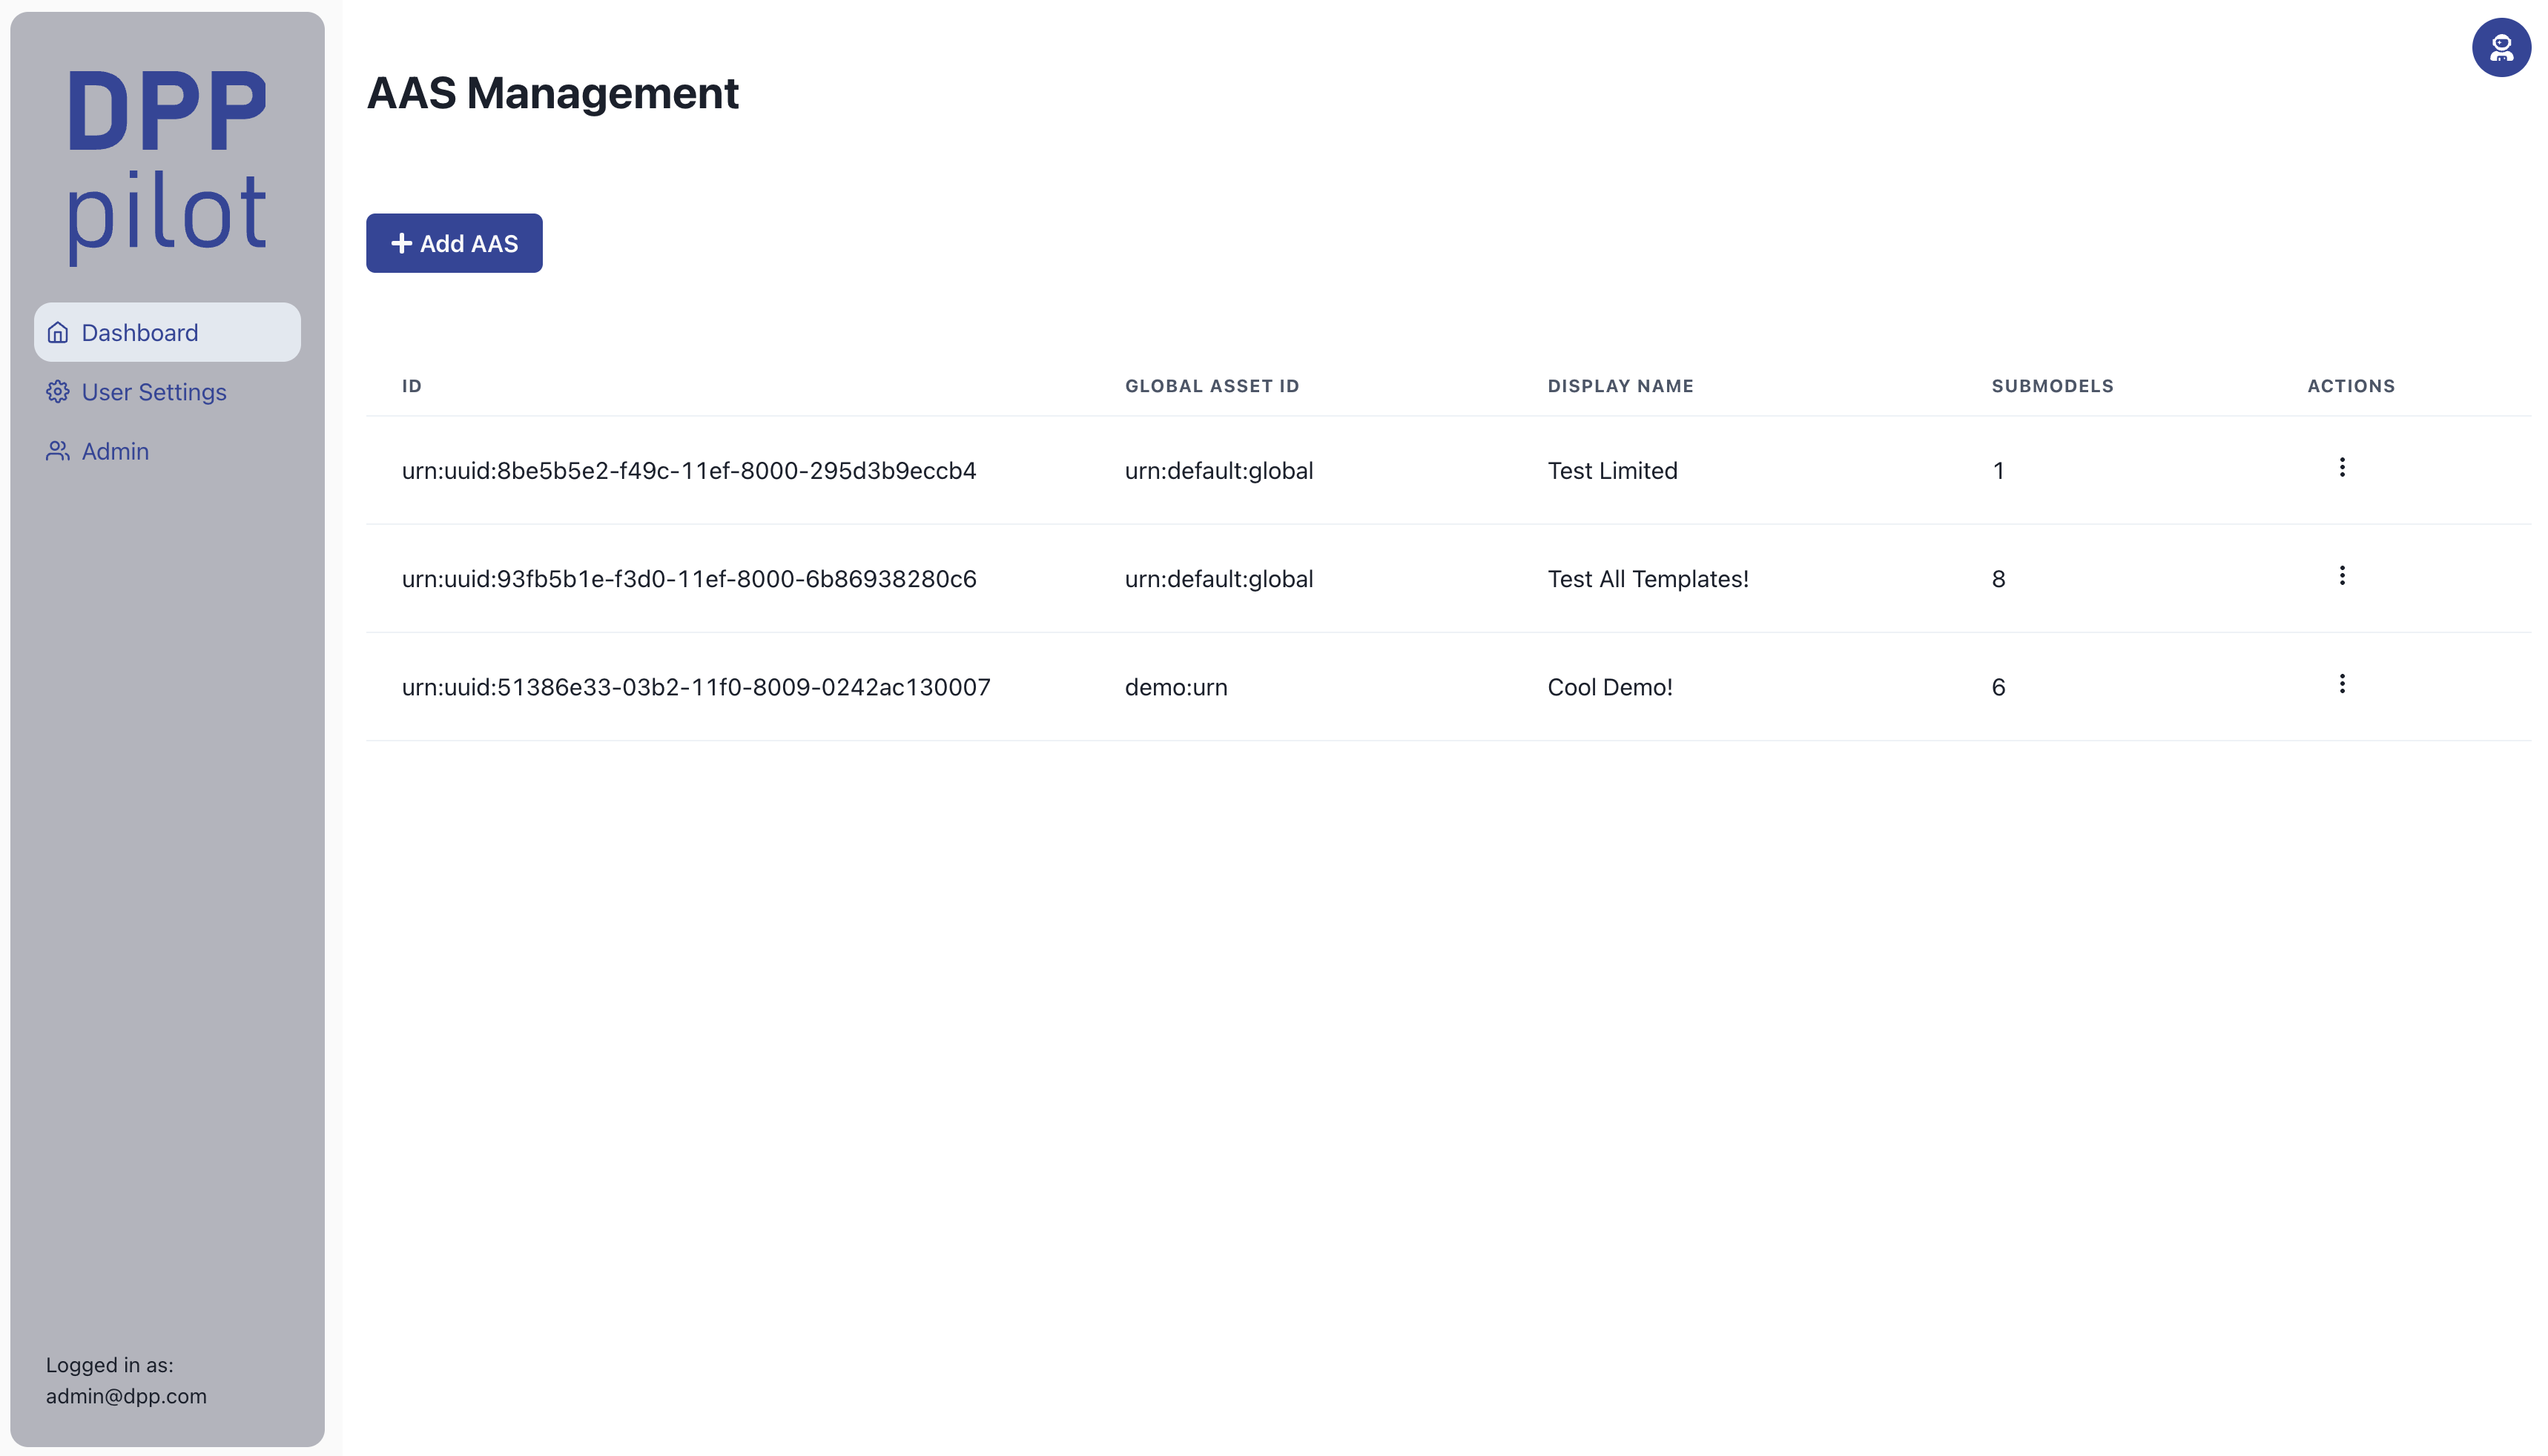
\includegraphics[width=\textwidth]{figures/pilot_interface_1.png}
  \caption{%
    \textit{\ac{aas} Management Dashboard: Main Interface} 
  }
  \label{fig:pilot_interface_1}
\end{figure}

\begin{figure}[H]
  \centering
  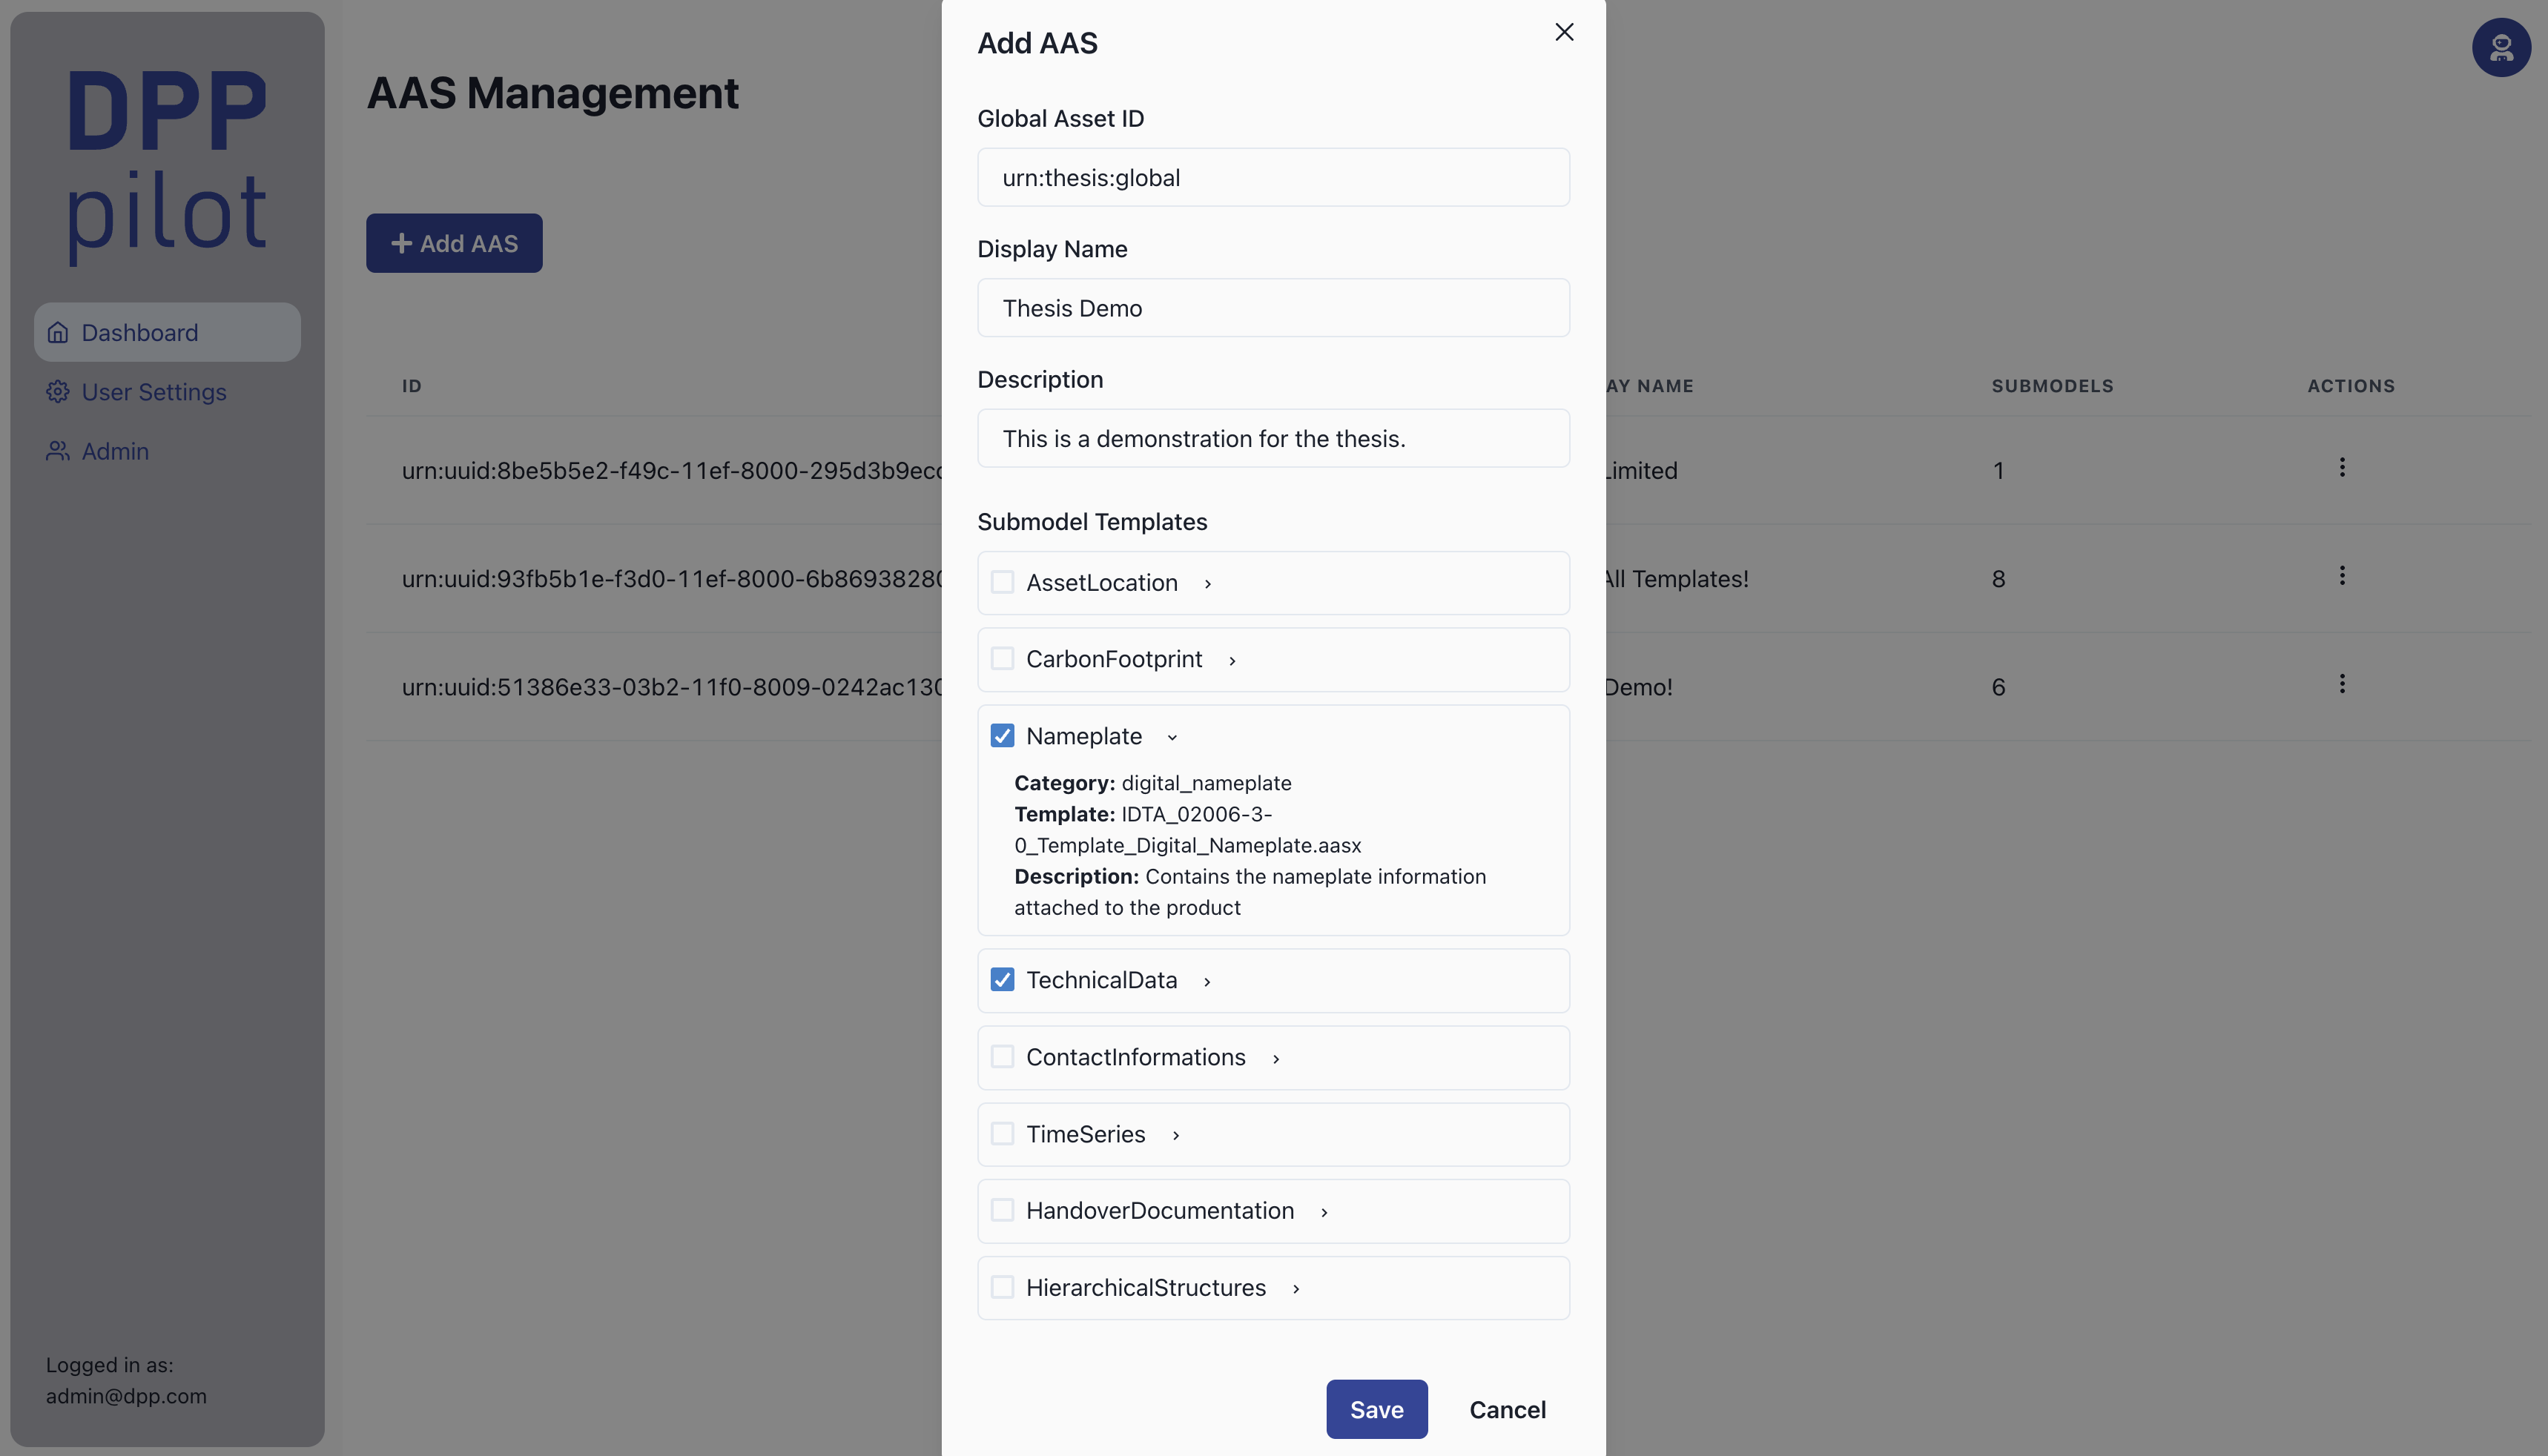
\includegraphics[width=\textwidth]{figures/pilot_interface_2.png}
  \caption{%
    \textit{\ac{aas} Management Dashboard: \ac{aas} Instance Creation} 
  }
  \label{fig:pilot_interface_2}
\end{figure}

\Cref{fig:pilot_interface_2}: \ac{aas} instantiation modal window, allowing administrators to configure metadata and select desired standardized submodel templates for dynamic instantiation.

\begin{figure}[H]
  \centering
  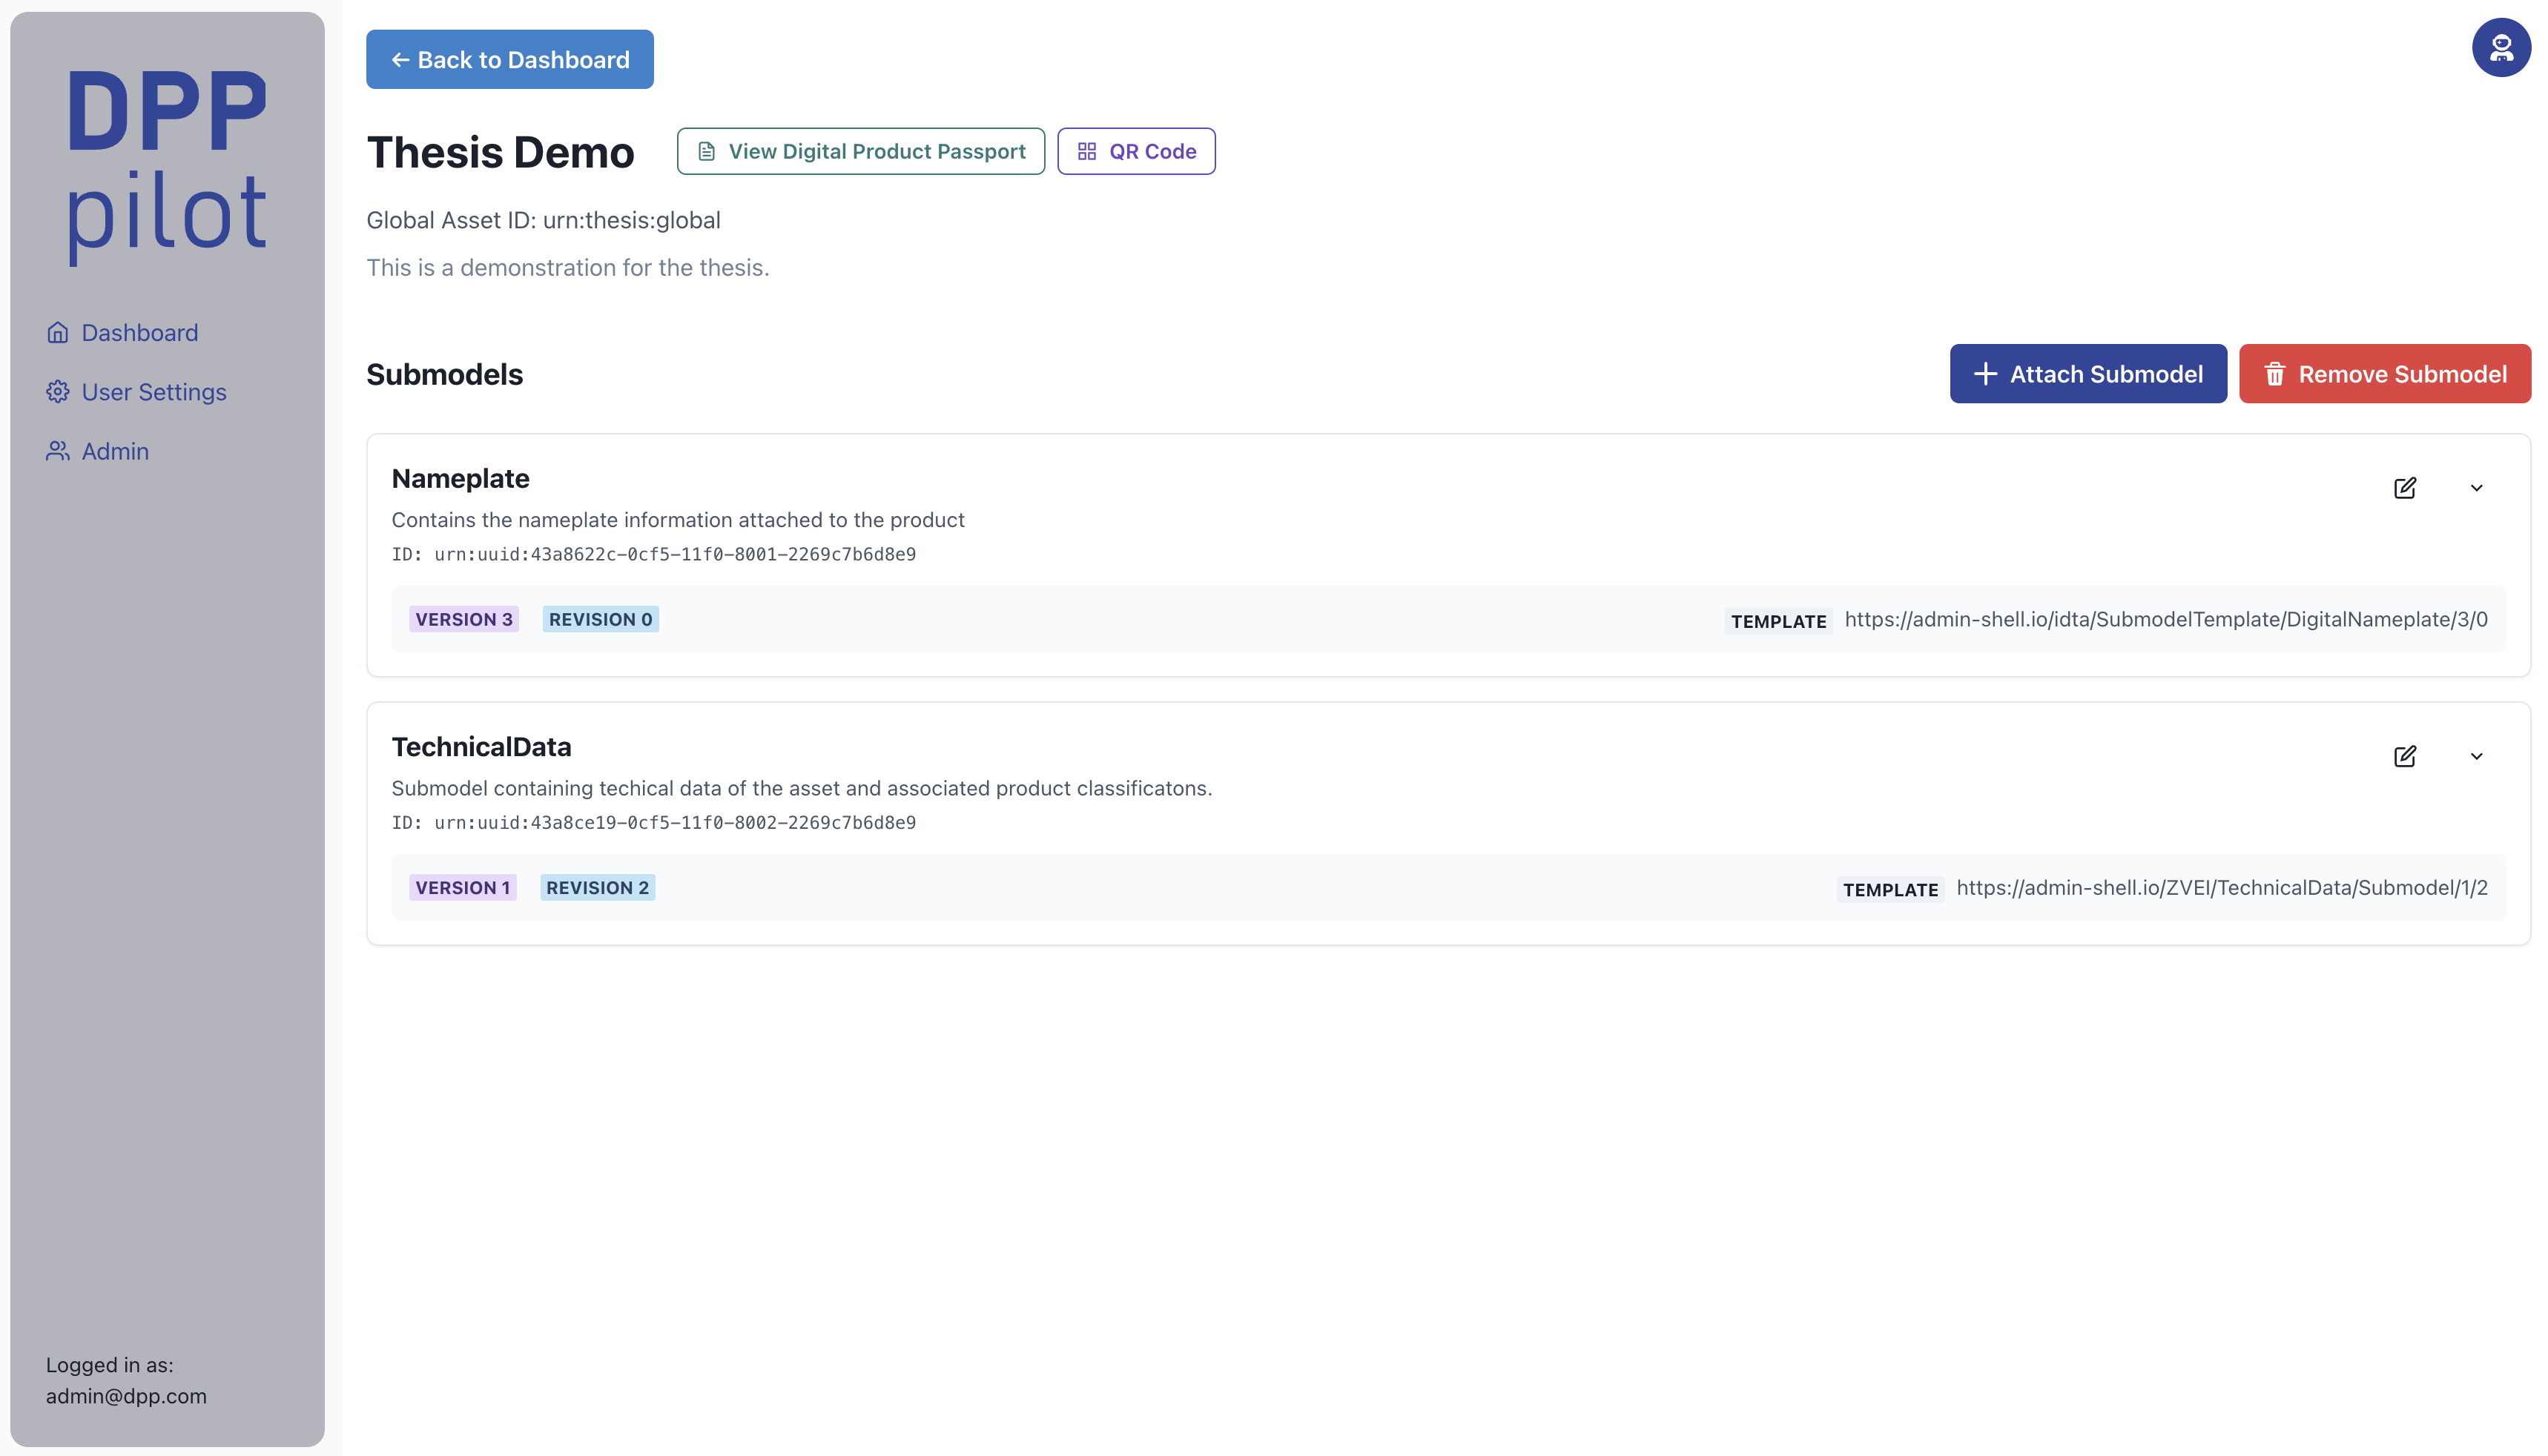
\includegraphics[width=\textwidth]{figures/pilot_interface_3.png}
  \caption{%
    \textit{\ac{aas} Management Dashboard: \ac{aas} Instance Overview Page} 
  }
  \label{fig:pilot_interface_3}
\end{figure}

\Cref{fig:pilot_interface_3}: Detailed \ac{aas} instance overview page, showing metadata and associated submodels, with capabilities for submodel attachment, removal, property editing, and direct access to the generated \ac{dpp}. Note that submodel attachment and removal are restricted to administrator users, while employees can view and manage data.

\begin{figure}[H]
  \centering
  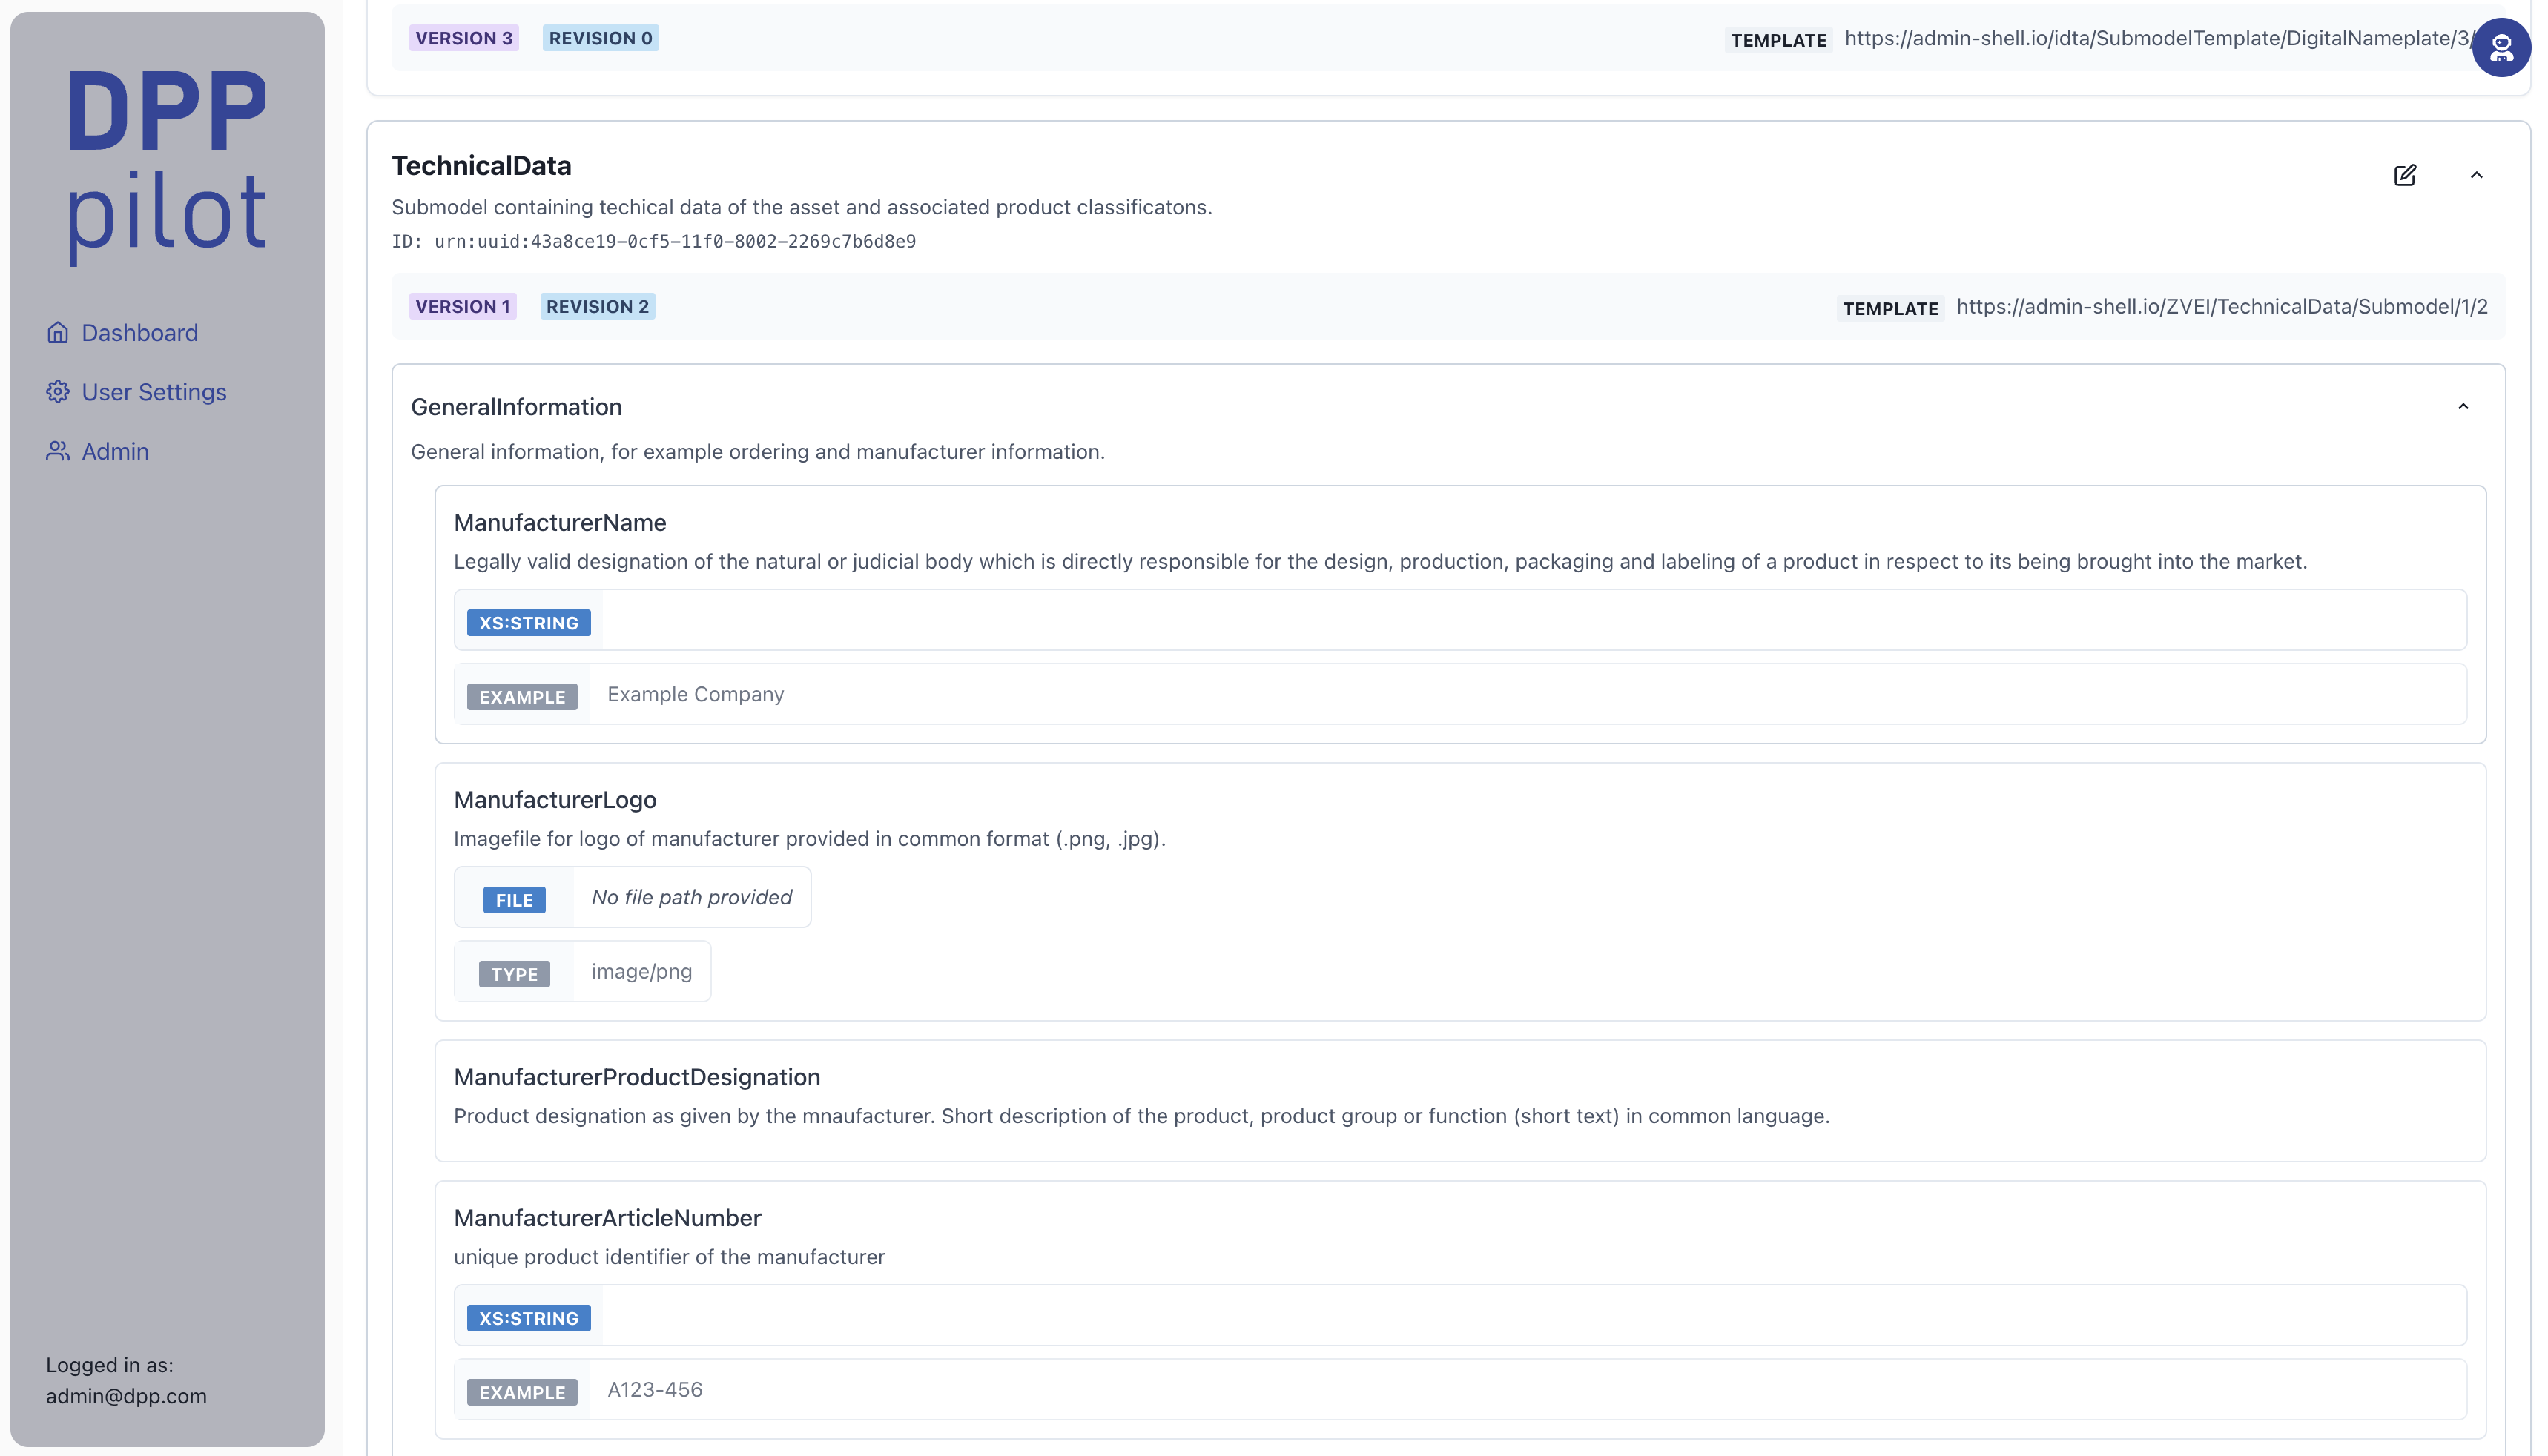
\includegraphics[width=\textwidth]{figures/pilot_interface_5.png}
  \caption{%
    \textit{\ac{aas} Management Dashboard: Submodel View Mode} 
  }
  \label{fig:pilot_interface_5}
\end{figure}

\Cref{fig:pilot_interface_5}: \ac{aas} submodel view mode interface, displaying structured, standardized elements defined by the \ac{idta} submodel template (e.g., Technical Data), presented clearly to allow users to review existing asset information.

\begin{figure}[H]
  \centering
  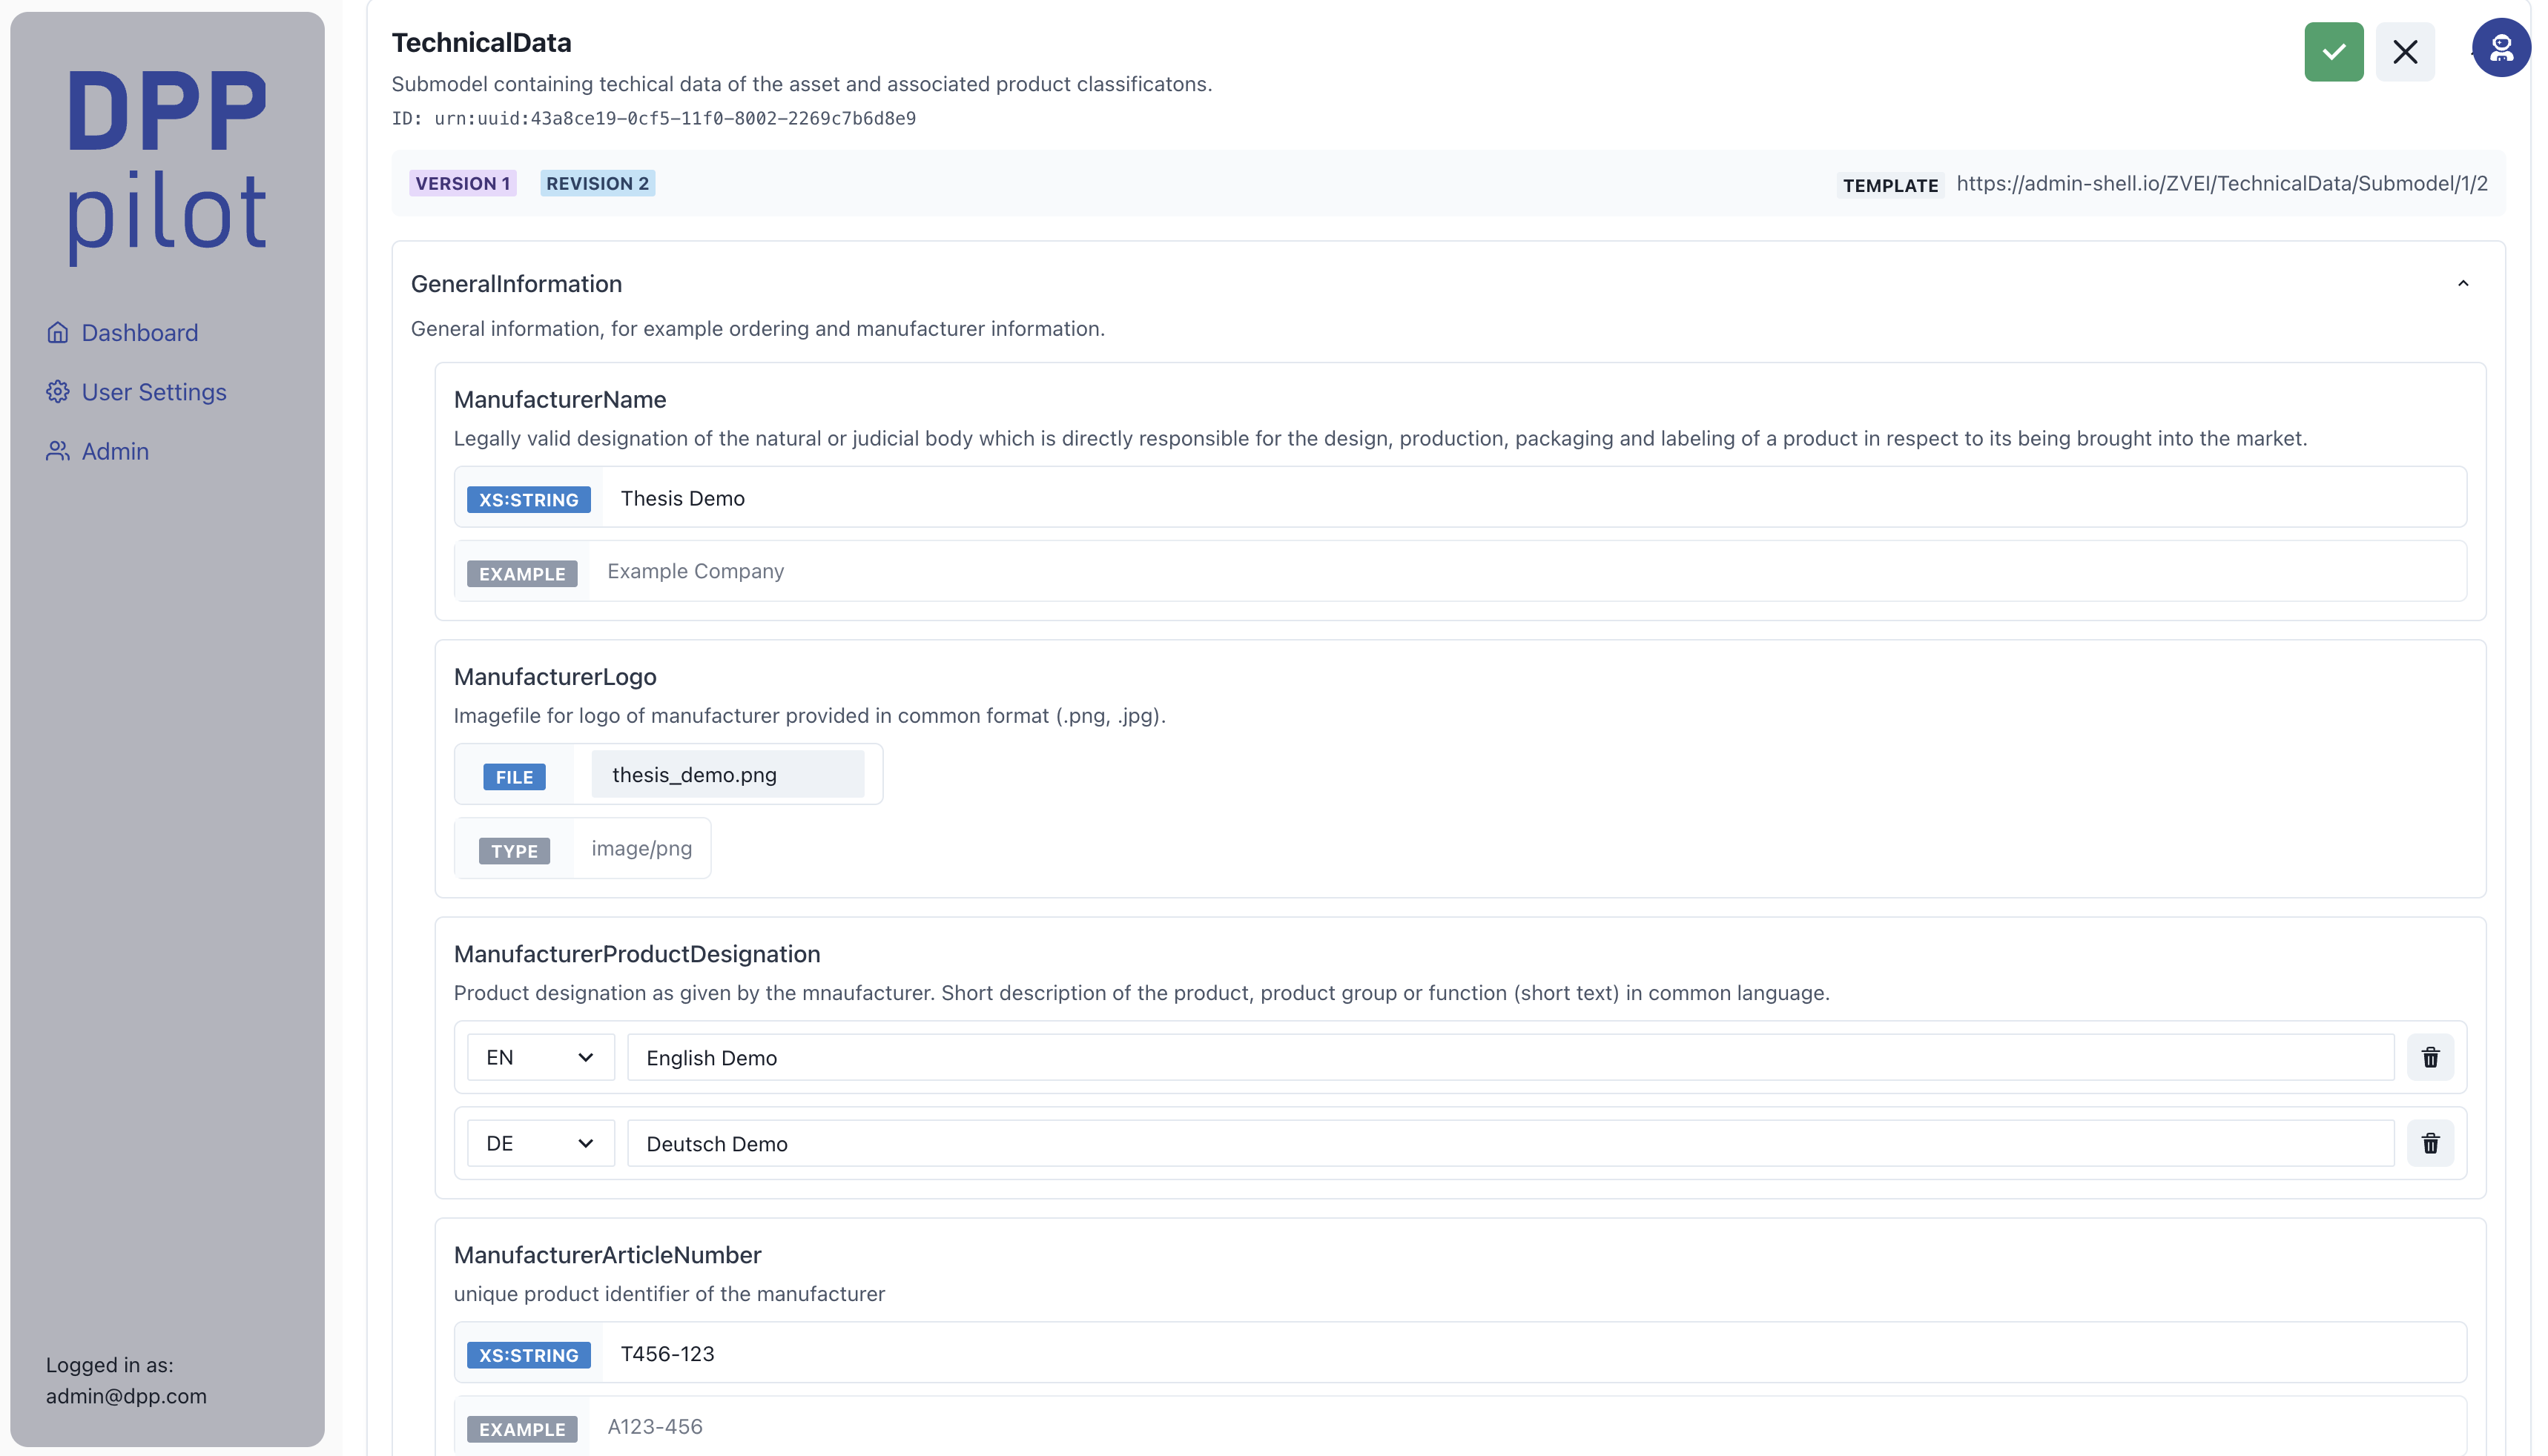
\includegraphics[width=\textwidth]{figures/pilot_interface_6.png}
  \caption{%
    \textit{\ac{aas} Management Dashboard: Submodel Edit Mode} 
  }
  \label{fig:pilot_interface_6}
\end{figure}

\Cref{fig:pilot_interface_6}: \ac{aas} submodel edit mode interface, enabling administrators and authorized users (e.g., employees) to directly update properties, manage multilingual content, and upload relevant files.

\begin{figure}[H]
  \centering
  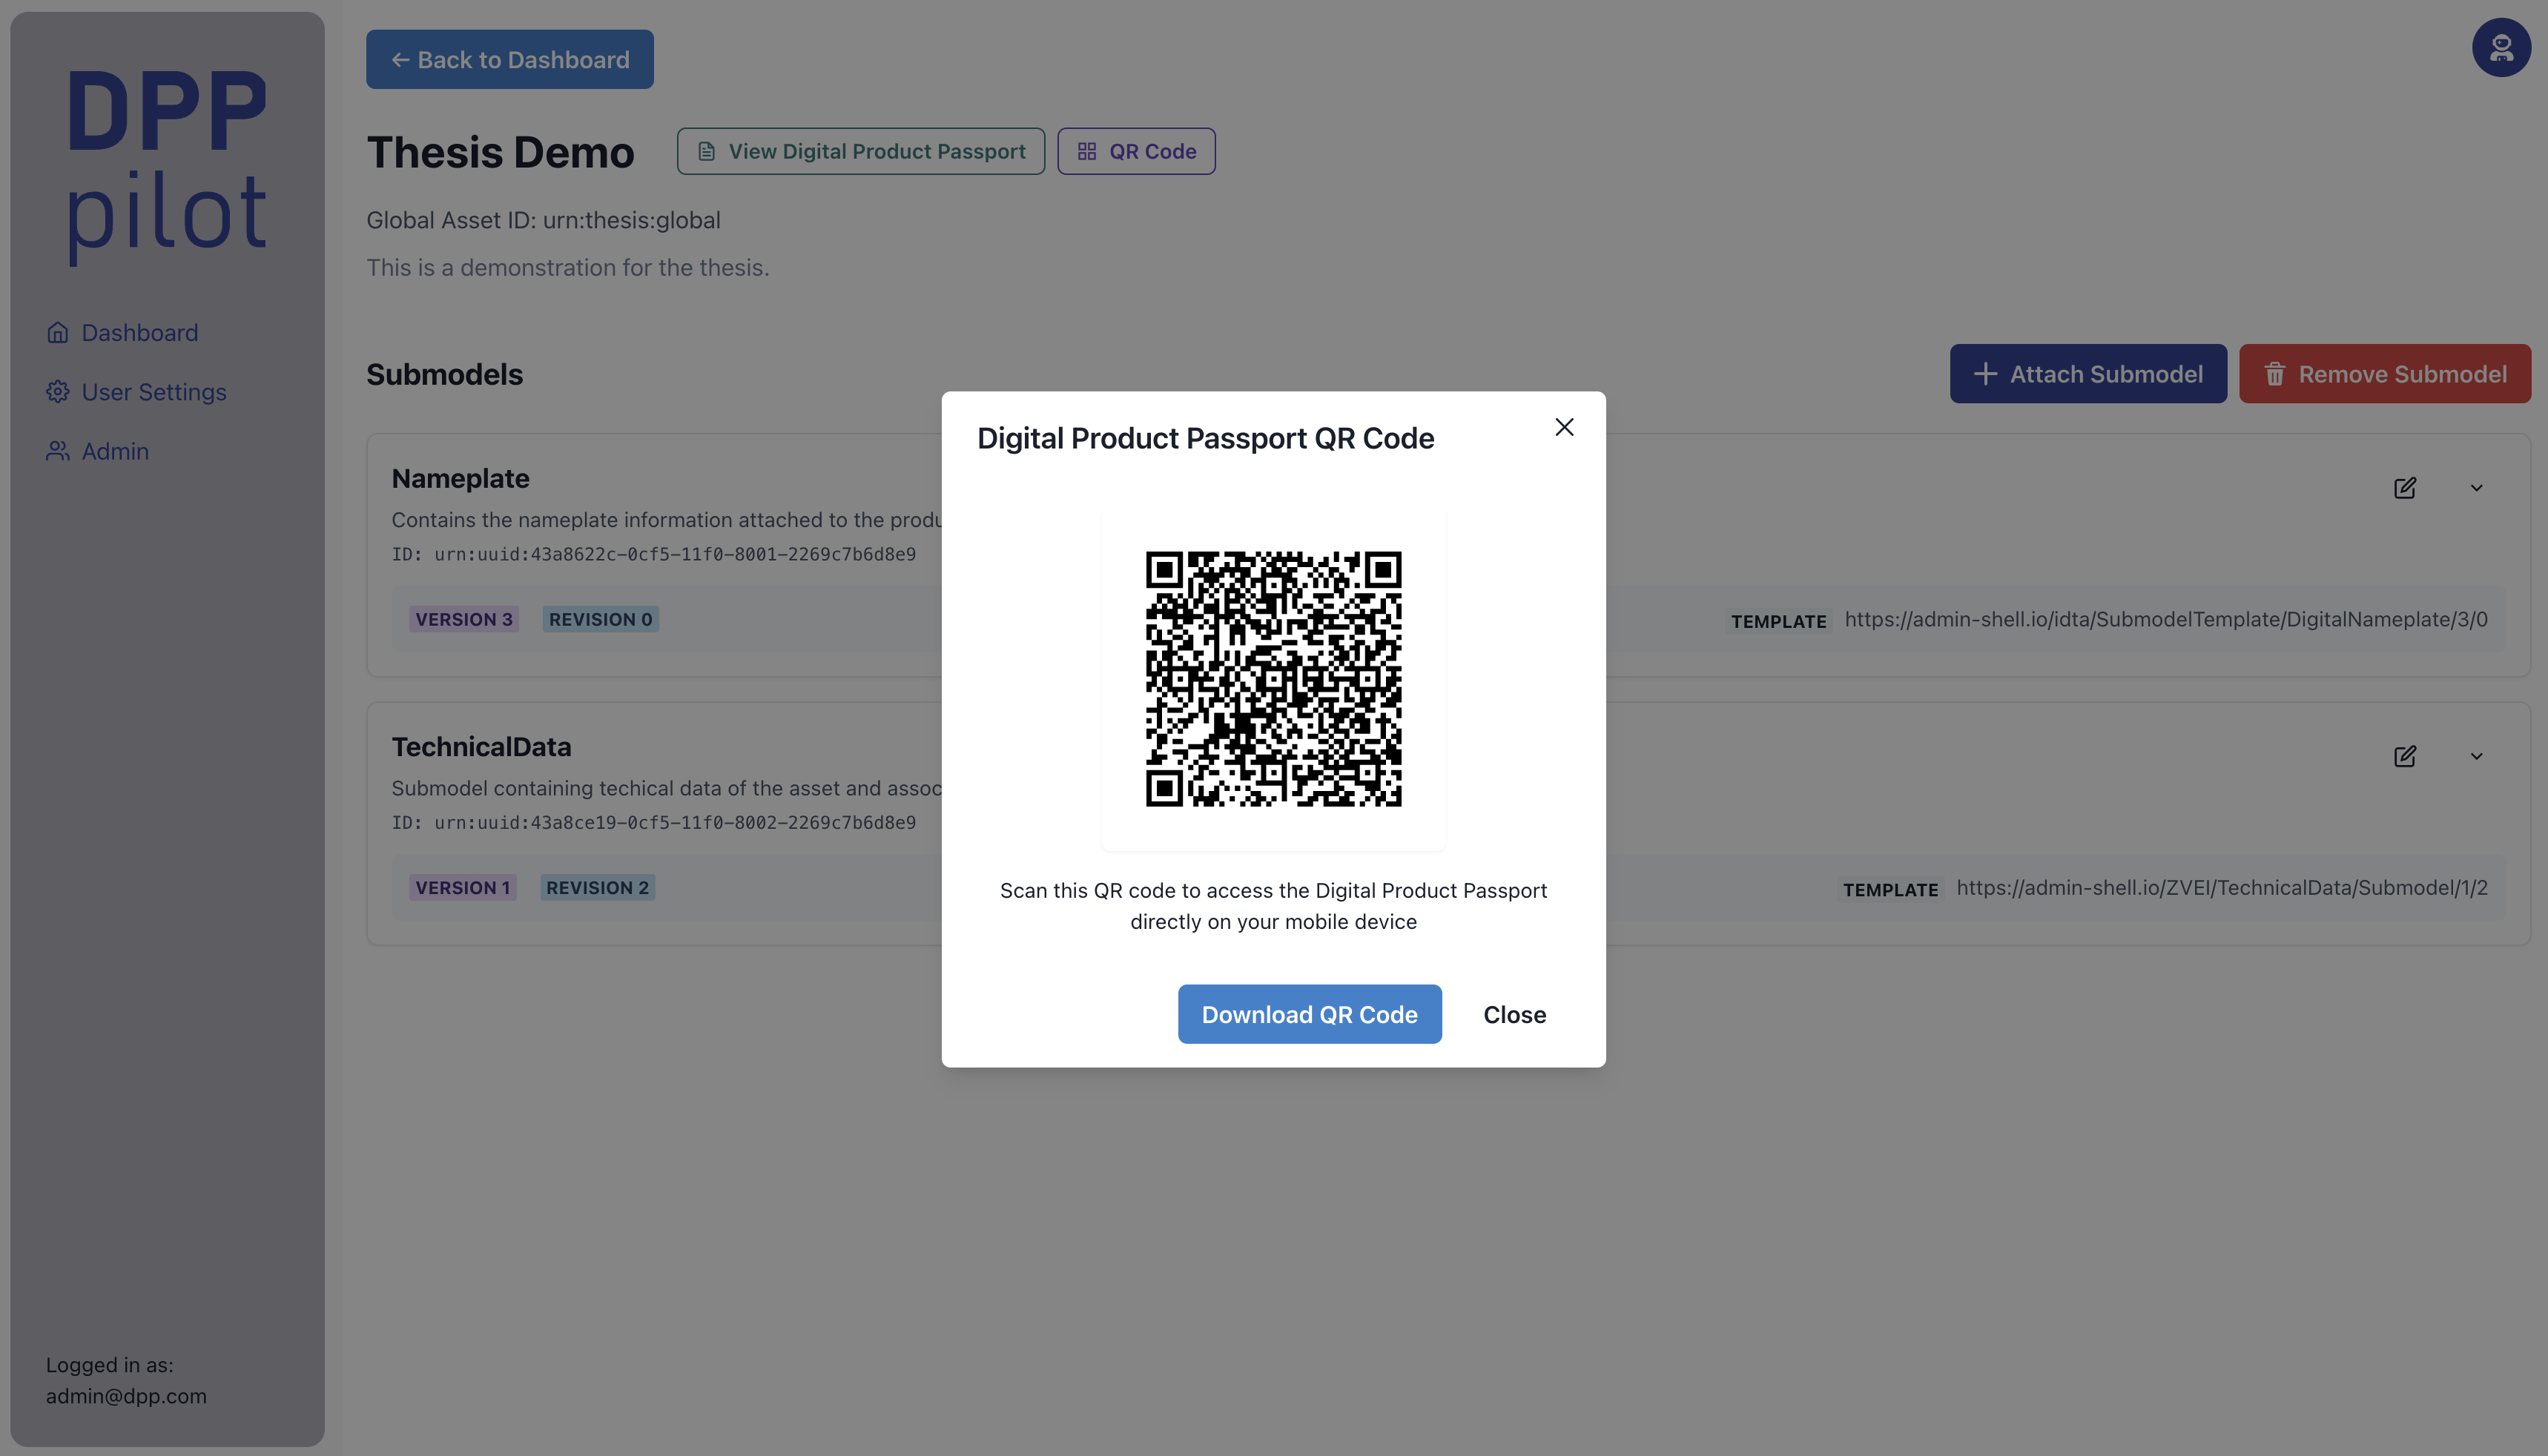
\includegraphics[width=0.8\textwidth]{figures/pilot_interface_4.png}
  \caption{%
    \textit{\ac{aas} Management Dashboard: \ac{dpp} \ac{qr} Code} 
  }
  \label{fig:pilot_interface_4}
\end{figure}

\Cref{fig:pilot_interface_4}: The \ac{dpp} \ac{qr} code generation and download feature provides immediate mobile access to the public-facing \ac{dpp} view, enabling employees to verify the \ac{dpp} mapping and quickly retrieve the \ac{qr} code for their product.

\begin{figure}[htbp]
    \centering
    \begin{minipage}{0.48\textwidth}
        \centering
        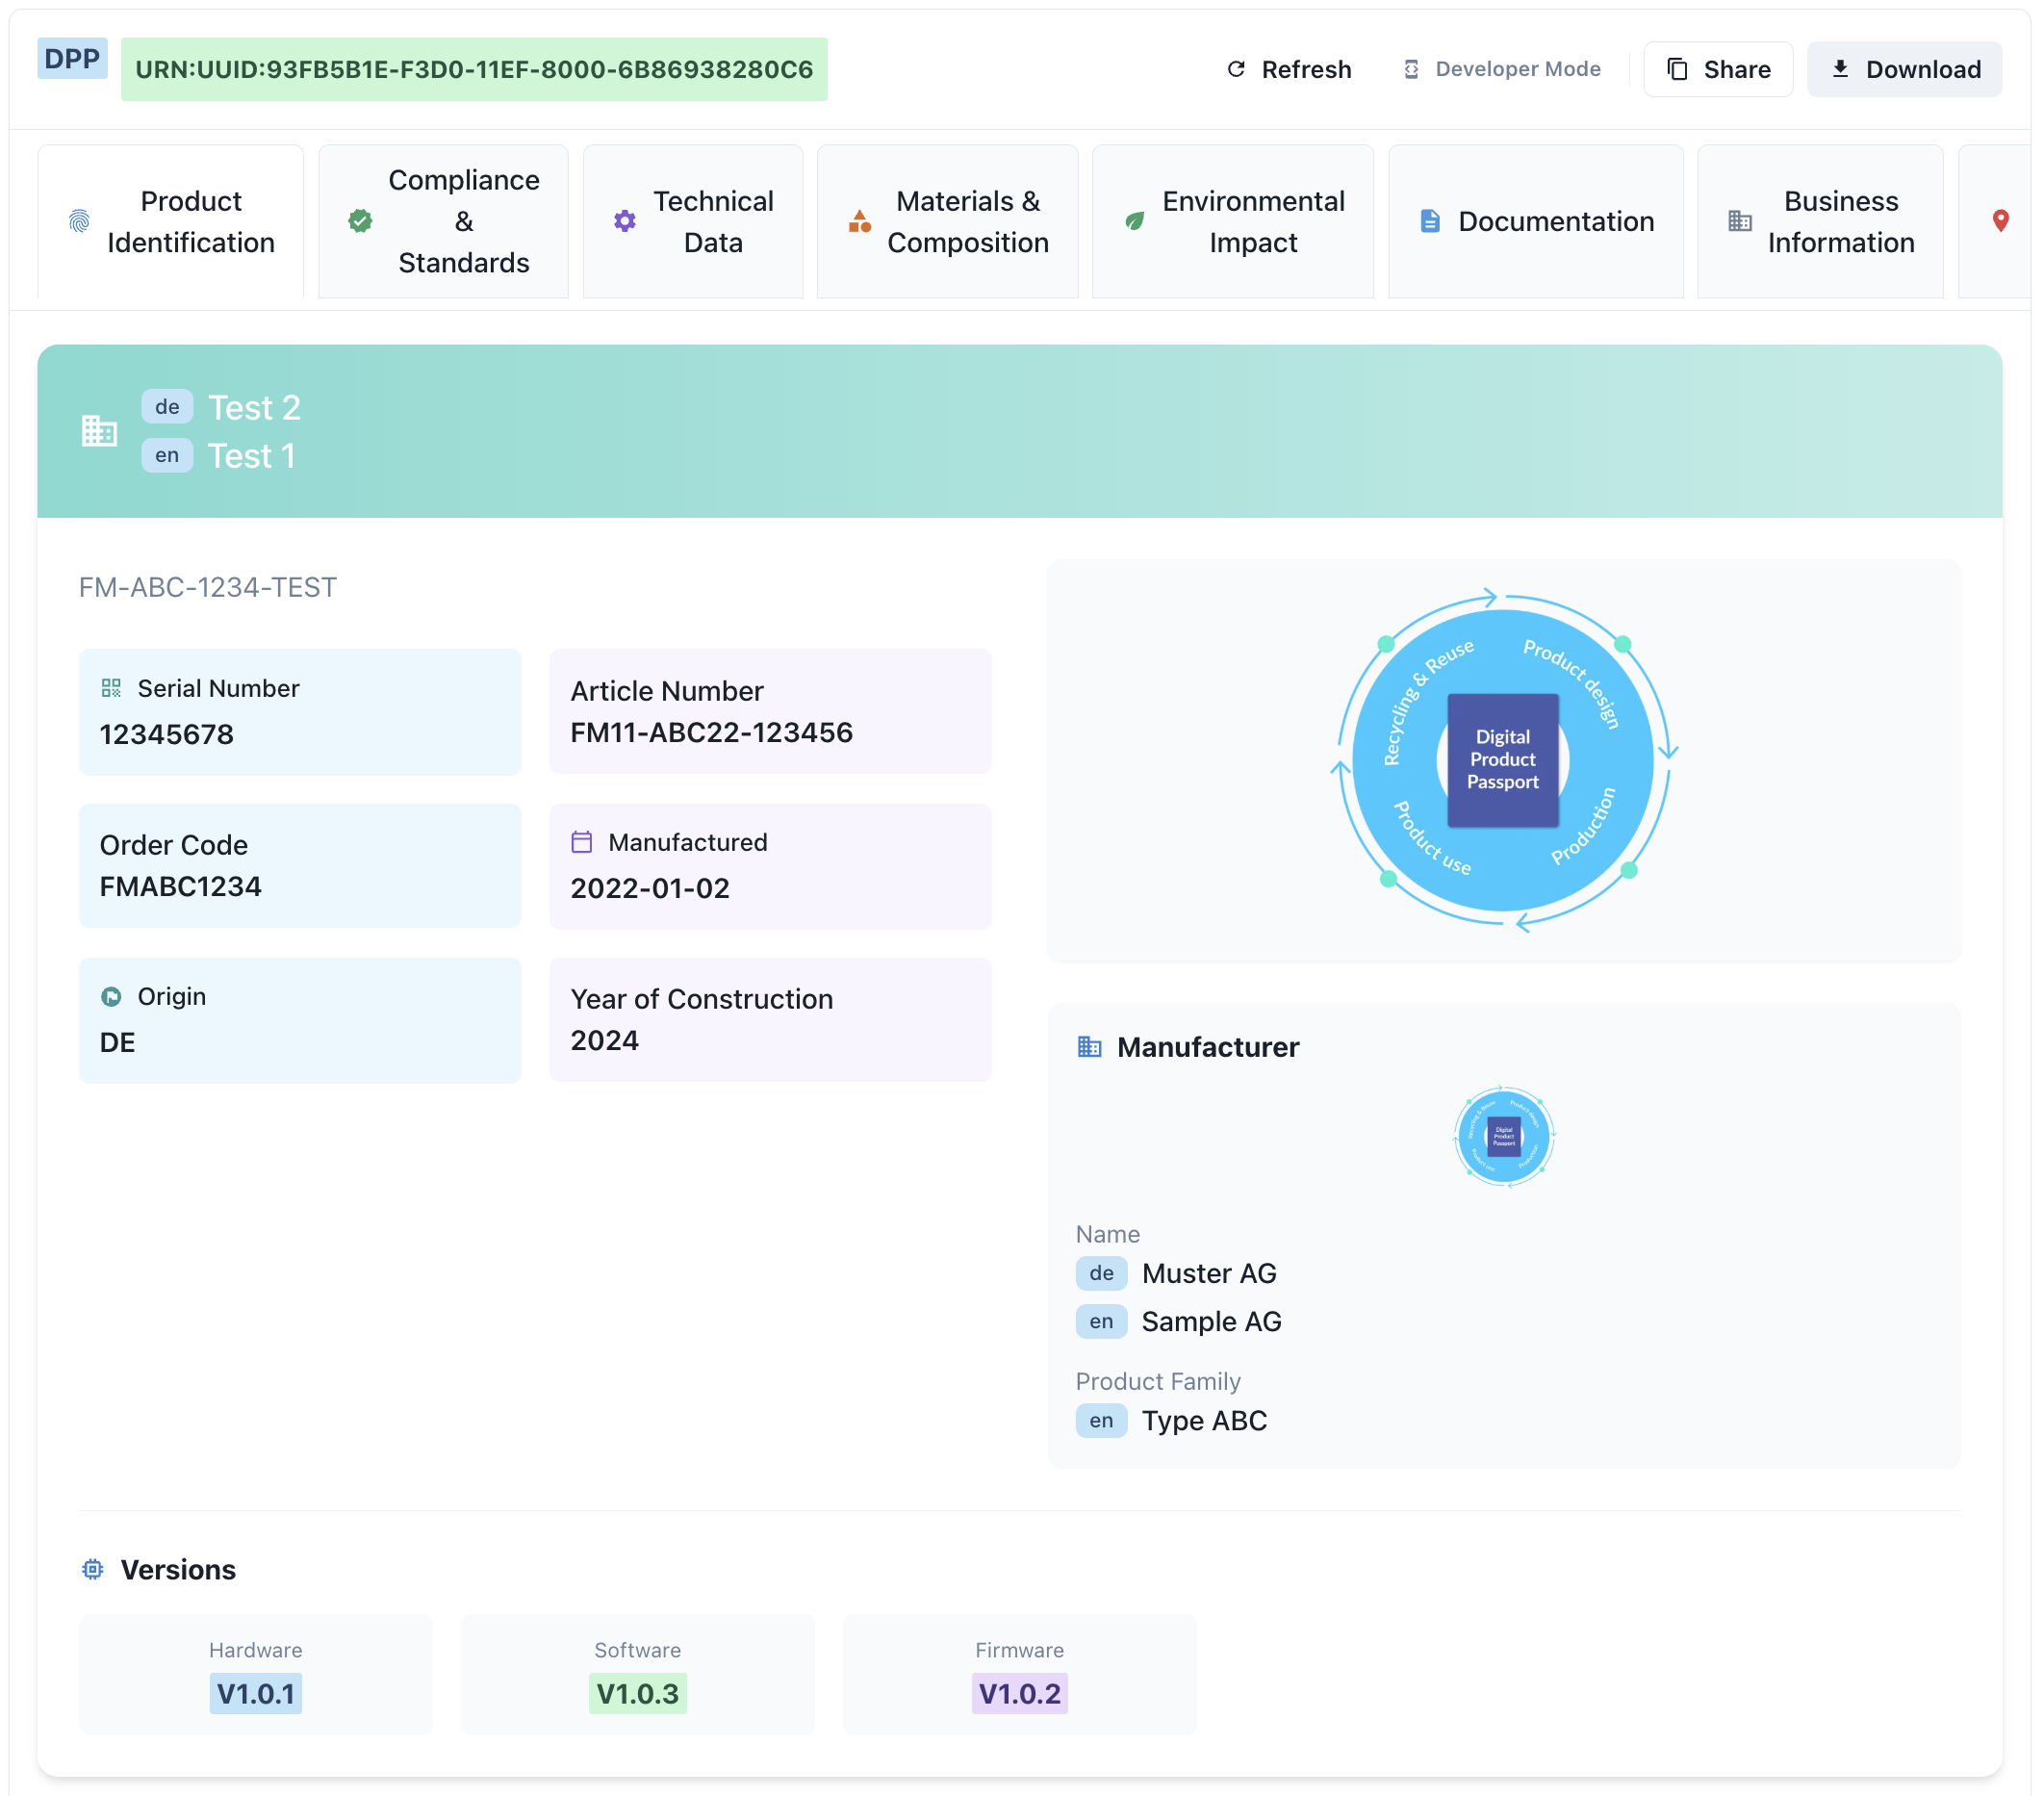
\includegraphics[width=\linewidth]{figures/pilot_interface_7.png}
        \caption{%
            \textit{\ac{dpp} Viewer: Identification Section} 
        }
        \label{fig:pilot_interface_7}
    \end{minipage}
    \hfill
    \begin{minipage}{0.48\textwidth}
        \centering
        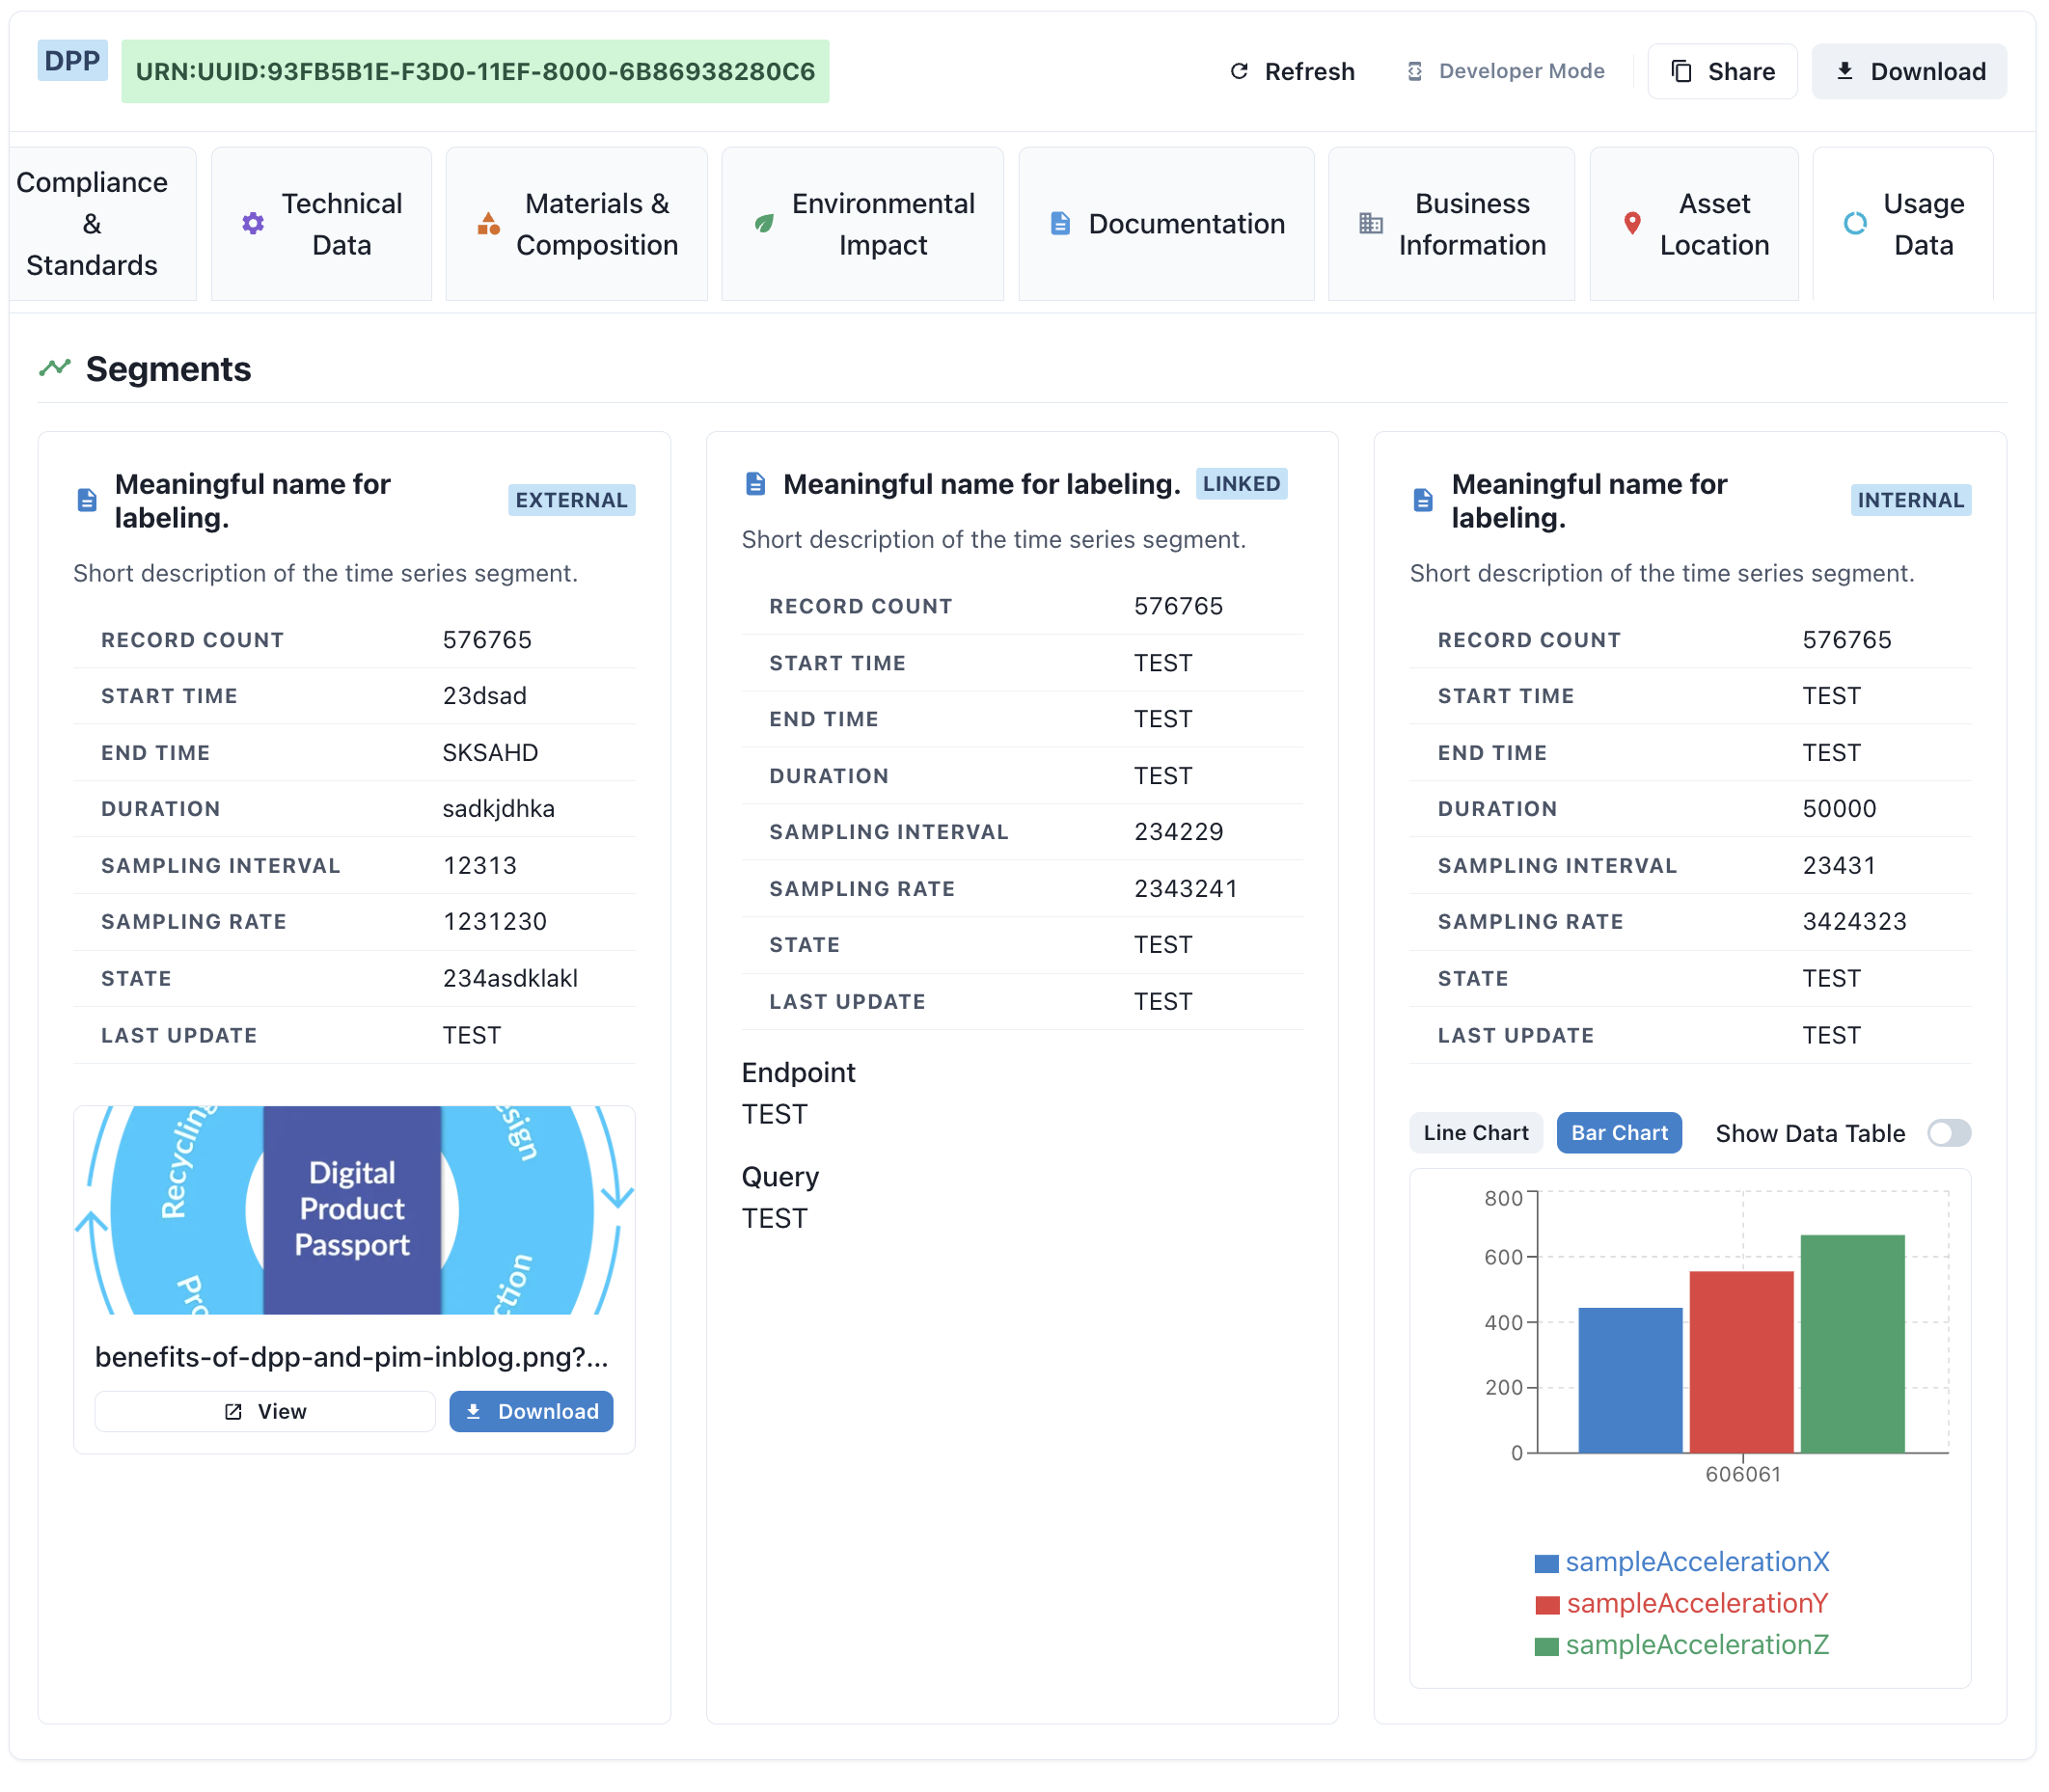
\includegraphics[width=\linewidth]{figures/pilot_interface_8.png}
        \caption{%
            \textit{\ac{dpp} Viewer: Usage Data Section} 
        }
        \label{fig:pilot_interface_8}
    \end{minipage}
\end{figure}

\begin{figure}[H]
  \centering
  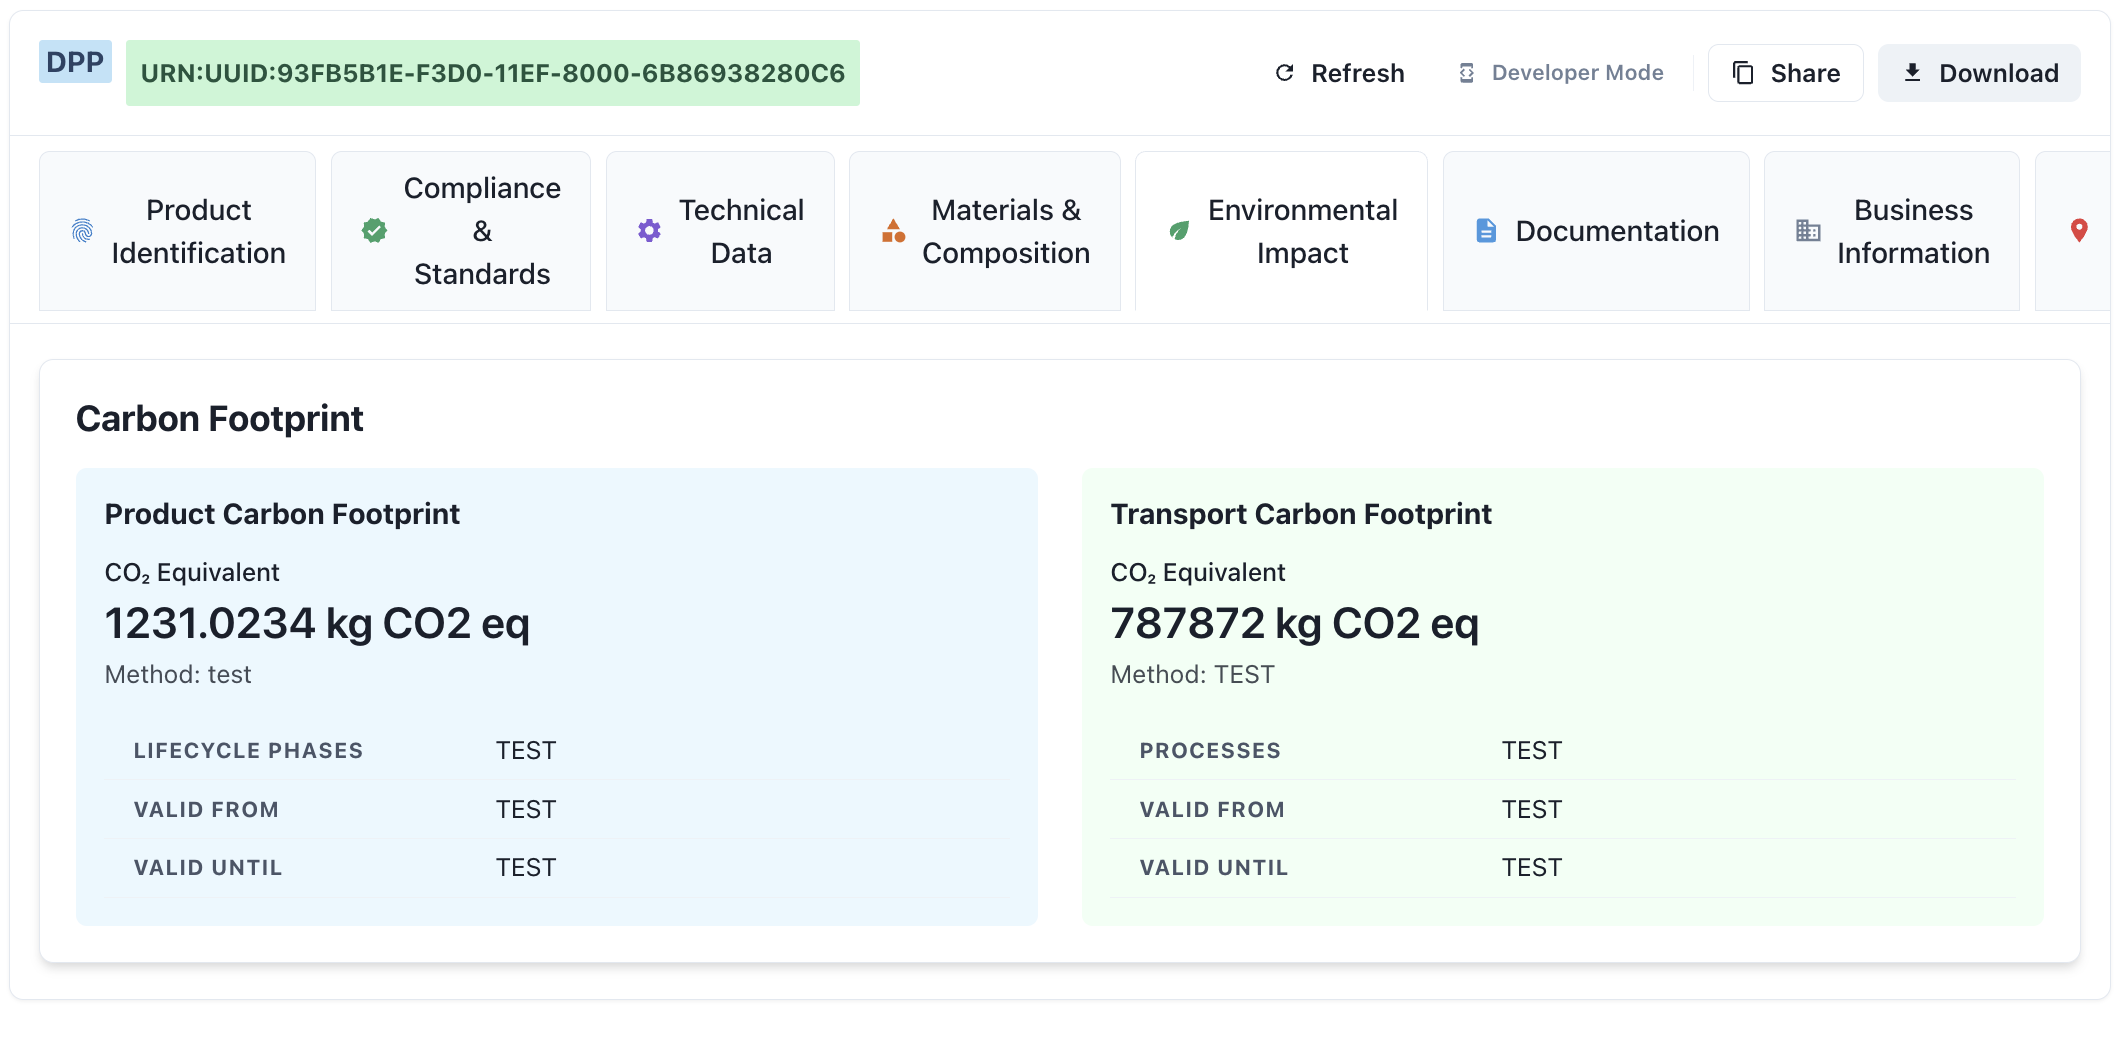
\includegraphics[width=\textwidth]{figures/pilot_interface_9.png}
  \caption{%
    \textit{\ac{dpp} Viewer: Environmental Impact Section} 
  }
  \label{fig:pilot_interface_9}
\end{figure}

The \ac{dpp} Viewer module is publicly accessible and provides an intuitive, structured representation of the product data derived from the corresponding \ac{aas} instance. \Cref{fig:pilot_interface_7,fig:pilot_interface_8,fig:pilot_interface_9} demonstrate selected sections of the generated \acrlong{dpp} interface. Specifically, \Cref{fig:pilot_interface_7} illustrates the Product Identification section, showcasing essential product data such as serial number, manufacturing details, and manufacturer information. \Cref{fig:pilot_interface_8} highlights the Environmental Impact section, providing clear visualizations of carbon footprint metrics for the product's lifecycle phases. Finally, \Cref{fig:pilot_interface_9} exemplifies the Usage Data section, integrating dynamic visual elements such as interactive charts to effectively communicate time series data related to product usage and operational statistics. The modular and dynamic nature of the \ac{dpp} Viewer ensures both semantic clarity and comprehensive data accessibility for varied stakeholders.